\documentclass[a4paper, 12pt]{report}
%    \renewcommand{\baselinestretch}{1.6}      % interline spacing
%
% \includeonly{}
%
%			PREAMBOLO
%
\usepackage[a4paper]{geometry}
\usepackage{amssymb,amsmath,amsthm}
\usepackage{graphicx}
\usepackage{url}
\usepackage{hyperref}
\usepackage{epsfig}
\usepackage[english]{babel}
\usepackage{setspace}
\usepackage{tesi}
\usepackage{listings}

\usepackage{pifont}% http://ctan.org/pkg/pifont
\newcommand{\cmark}{\ding{51}}%
\newcommand{\xmark}{\ding{55}}%


% per le accentate
\usepackage[utf8]{inputenc}
%
\newtheorem{myteor}{Teorema}[section]
%
\newenvironment{teor}{\begin{myteor}\sl}{\end{myteor}}
%
%Path relative to the main .tex file 
\graphicspath{ {./images/} }
%
%			TITOLO
%
\begin{document}
\title{Design and development of an assurance methodology for security certifications in IoT systems}
\author{Matteo CAVAGNINO}
\dept{Corso di Laurea in Informatica} 
\anno{2021-2022}
\matricola{961707}
\relatore{Prof. Claudio ARDAGNA}
\correlatore{Dr. Nicola BENA}
%
%        \submitdate{month year in which submitted to GPO}
%		- date LaTeX'd if omitted
%	\copyrightyear{year degree conferred (next year if submitted in Dec.)}
%		- year LaTeX'd (or next year, in December) if omitted
%	\copyrighttrue or \copyrightfalse
%		- produce or don't produce a copyright page (false by default)
%	\figurespagetrue or \figurespagefalse
%		- produce or don't produce a List of Figures page
%		  (false by default)
%	\tablespagetrue or \tablespagefalse
%		- produce or don't produce a List of Tables page
%		  (false by default)
% 
%			DEDICA
%
\beforepreface
\prefacesection{}
        {\hfill \Large {\sl dedicato a \dots}}
% 
%			PREFAZIONE
%
\prefacesection{Preface}
hkjafgyruet.
%
%
%			ORGANIZZAZIONE
\section*{Organization of the thesis}
\label{organizzazione}
The thesis is organized as follows:
\begin{itemize}
\item in Chapter 1 ....
\end{itemize}
%
%			RINGRAZIAMENTI
%
\prefacesection{Acknowledgements}
asdjhgftry.
\afterpreface
% 
% 
%			CAPITOLO 1: Introduzione
\chapter{Introduction}
\label{cap1}                        % riferire al capitolo con \ref{cap1}



\chapter{State Of The Art}
\label{cap2}
This chapter introduces the main system paradigms that today guide the various security certification frameworks.

\section{Cloud Computing Paradigm}
The National Institute of Standards and Technology (NIST) defined the Cloud computing paradigm as follows: “Cloud computing is a model for enabling ubiquitous, convenient, on-demand network access to a shared pool of configurable computing resources (e.g., networks, servers, storage, applications, and services) that can be rapidly provisioned and released with minimal management effort or service provider interaction \cite{mell2011nist}."

The most commonly used deployment model for Cloud computing is the public Cloud, which allows users to access its resources through the Internet and is generally subject to monetization from provider companies.
Another commonly used deployment model is the private Cloud, usually found in single organizations for a more secure digital environment.
The other two models are Hybrid Cloud and Community Cloud, where the former is a mixture of public and private Cloud that overcomes some of the limitations of each, and the latter is an expansion from a private cloud, allowing multiple organizations to access its resources \cite{atlam2017integration}.

The essential services that Cloud computing offers include infrastructure as a service (IaaS), platform as a service (PaaS) and software as a service (SaaS), each of whom allows a different calibre of resources' control between the user and the provider \cite{khan2019edge}.

%%%%%%%%%%%%%%%%%%%%%%%%%%%%%%%%%%%%%%%%%%%%%%%%%%%%%%%%%%%%%%%%%%%%%%%%%%%%%%

\subsection{IoT in Cloud Environments}
Given the general flexibility, dynamicity and resource availability of Cloud computing, it has been the first adopted solution for IoT (Internet of Things) systems implementations.
The IoT label defines the network created around small smart devices interconnected through the Internet. To be classified as an IoT device, a piece of hardware has to be embedded with electronics, software, and connectivity in a way that enables it to communicate with other devices and exchange data that can be directly gathered from the device itself thanks to specific embedded sensors or from other connected devices.
The range of possible objects that today are intended as Smart IoT devices is vast; it comprehends instruments, vehicles, buildings, all sorts of sensor-enabled devices \cite{gokhale2018introduction}, industrial machines, and small objects like clothing, packages, parts, materials and much more. All these objects are active participants in the network and thus can be monitored, tracked and counted.
Cloud computing and IoT are built with complementary ideas; on the one hand, the Cloud is ubiquitous, secure, flexible and equipped with such a broad resource capability that it is often referred to as infinite. However, on the other hand, IoT devices are distributed and capable of generating immense moles of data that need a powerful computing element to analyze and process them.
Cloud computing simplifies the IoT data flow significantly and helps overcome many devices' limitations such as security, privacy, performance, and reliability. The main benefits of IoT integration in Cloud environments are widely discussed in \cite{atlam2017integration}.

As mentioned above, IoT devices generate a significant constant flow of data that for sure cannot be handled by the small devices themselves, but that is also becoming an issue for the Cloud infrastructures since IoT systems grow bigger and bigger every year, with more sensors and more communicating units [need source].
The biggest challenge in the IoT field is managing the massive quantity of data generated, and even the Cloud solutions are challenged by the large scale, heterogeneity and high latency issues. One rapidly increasing solution in popularity consists of using a decentralized computing model known as Fog Computing \cite{iorga2018fog}.

%%%%%%%%%%%%%%%%%%%%%%%%%%%%%%%%%%%%%%%%%%%%%%%%%%%%%%%%%%%%%%%%%%%%%%%%%%%%%%

\section{Edge Computing Paradigm}
\label{Edge}
Edge computing directs computational data, applications, and services away from Cloud servers to the edge of a network (figure \ref{fig:ceiot_stack}). The content providers and application developers can use the Edge computing systems by offering the users services closer to them. Edge computing is characterized in terms of high bandwidth, ultra-low latency, and real-time access to the network information that can be used by several applications \cite{khan2019edge}.

Edge or Fog computing is the latest and most promising researched solution to the recent trends of distributing the computation closer to the data sources. The goal is to provide low latency, high capacity and network efficient computation to IoT systems bringing multiple small Cloud nodes (Fog nodes) between the Cloud and the IoT devices at the "edge" of the network. As for many concepts, the definitions are numerous \cite{sahni2018data} but Yi et al. stated the following as a possible definition: "Fog Computing is a geographically distributed computing architecture with a resource pool which consists of one or more ubiquitously connected heterogeneous devices (including edge devices) at the edge of the network and not exclusively seamlessly backed by Cloud services, to collaboratively provide elastic computation, storage and communication (and many other new services and tasks) in isolated environments to a large scale of clients in proximity" \cite{yi2015fog}.
Practically Fog computing represents an extension of Cloud computing that offers multiple benefits to the latter:

\begin{itemize}
    \item Location awareness and low latency
    \item Geographical distribution
    \item Scalability
    \item Support for mobility
    \item Real-time interactions
    \item Heterogeneity
    \item Interoperability
    \item Support for online analytics and interplay with the Cloud
\end{itemize}

\begin{figure}[h]
    \centering
    \fbox{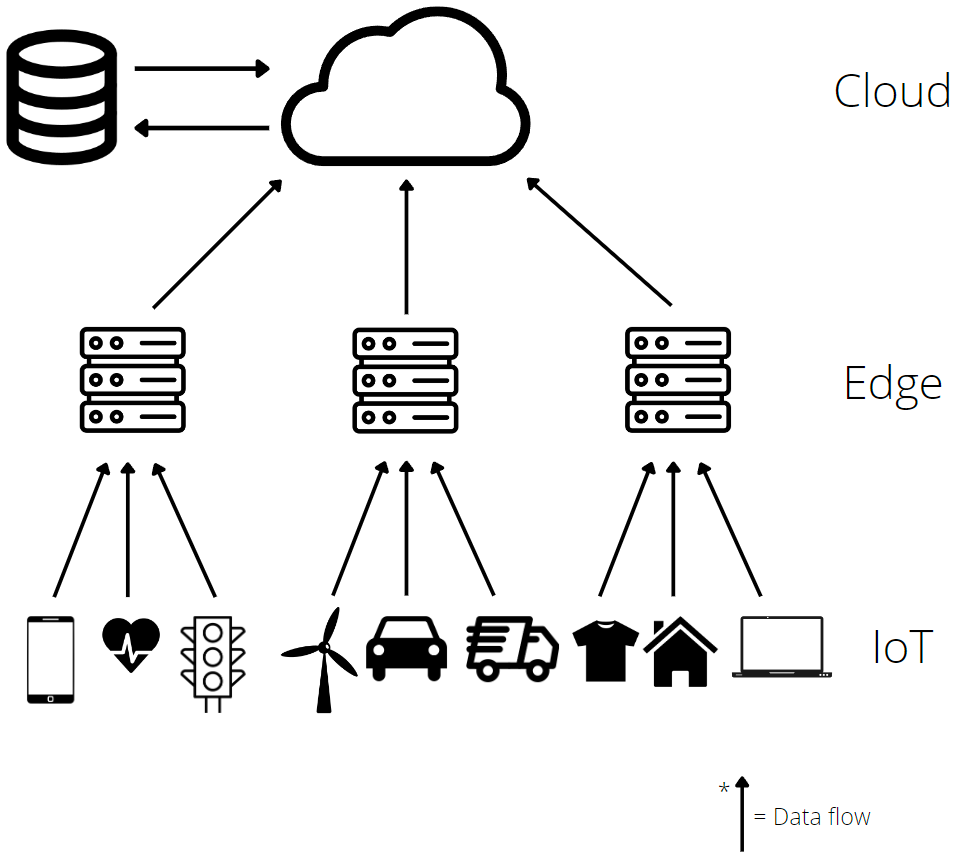
\includegraphics[scale=0.55]{images/cloud_edge_iot_stack.png}}
    \caption{Example of cloud-edge-IoT stack architecture}
    \label{fig:ceiot_stack}
\end{figure}

\subsection{Edge and Cloud Relationship}
Edge computing is considered an extension of Cloud computing and not a standalone computing paradigm; it still relies on the Cloud at the top level of its scheme, but it drastically reduces the load over the Cloud infrastructures while maintaining all of the Cloud's provided services like data computing, storage and applications. The main difference between the two is the location of the servers; with the Cloud alone, latency dependant applications may encounter latency and jitter issues due to the distance between the user device and the server. On the other hand, Edge computing enables location-aware and mobile applications with full support, while Cloud applications need to find other workarounds. The longer path to the server can also be a weak point for security attacks on the Cloud. Another difference is the target audience: Cloud computing is a global solution, Edge computing is limited. Lastly, the single Edge node hardware is designed to be horizontally scalable through distribution, while Cloud computing is generally more vertically scalable \cite{khan2019edge}.


Today, an ever-rising number of applications must use software that satisfies strict reliability, availability and integrity requirements, especially when dealing with critical safety systems; hence, multiple assurance and verification techniques have been introduced, such as certification schemes, testing, service level agreements, audit/compliance and monitoring frameworks \cite{ardagna2015security}. 


\section{Security and Assurance in Distributed Systems}
Software security assurance techniques enhance software and services transparency \cite{ardagna2014management} and increase the actors' confidence that such services behave as expected. In line with standard software security assurance definitions \cite{goertzel2007software}, cloud security assurance can be defined as the way to gain justifiable confidence that infrastructure and applications will consistently demonstrate one or more security properties and operationally behave as expected despite failures and attacks. However, assurance is a much wider notion than security, as it includes methodologies for collecting and validating evidence supporting security properties. When dealing with cloud infrastructure, Ardagna et al. \cite{article} highlighted three requirements that need to be considered with every assurance technique: i) risk assessment and management, ii) transparency and iii) public policy and compliance. 

Risk assessment and management are needed before the cloud service deployment and allow the business to obtain a precise evaluation of the risks that such a process would introduce. Transparency is a core component when defining and optimizing assurance techniques and allows end-users to visualize and control the data flow and the security issues in their services. In addition, transparency is necessary to support introspection, the capability of a cloud provider to examine and observe its internal processes, and outrospection, which is the same thing but from the customer's point of view \cite{ardagna2014management}. To comply with the transparency requirement, cloud providers must show their policies and compliance with standards and regulations and how such compliance is achieved \cite{macneil2006comply}. The major approaches to cloud assurance are discussed below.
\begin{description}
    \item[Testing]
    Testing involves executing software or system services with the help of manual or automated tools to evaluate specific behaviours and properties. The test activity allows gathering evidence to support the evaluation target's property; properties can belong to the cloud infrastructure or the service running on it.

    \item[Monitoring]
    Monitoring processes can be deployed to overcome the limits of direct testing approaches; it allows for gathering precise information about the status of services, events, and activities on the back end. In addition, the security of a cloud system can be greatly improved with monitoring approaches since they also increase transparency.

    \item[Certification]
    Various certification techniques have been developed to prove that a software system holds some non-functional properties and behaves as expected. The advantage of such techniques is the presence of a certificate released at the end of a successful process; such a certificate can then be shown as undisputable proof.
    
    \item[Audit and Compliance]
    An essential aspect of security and assurance is the capability of observing the system's behaviour and evaluating its compliance with customer policies and law regulations. Audit solutions have been developed with this very goal; additionally, they increase the system's transparency making systems like the cloud more accountable in case of issues and failures.
    
    \item[Service-Level Agreement (SLA)]
    SLA-based techniques establish contracts between clients and service providers, regulate their interactions, and model their expectations in functional and non-functional agreements \cite{article}.

\end{description}






\subsection{Security Certifications}
Security certifications are granted by independent (from the system supplier and acquirer) third parties whose goal is to verify the system's quality completely and objectively. Certifications allow more confidence in the product over the competition and legislative compliance when talking about quality, functionality and security \cite{heck2010software}. The certification schemes' main focus is to prove that the selected software system or service would have some non-functional properties and behave as expected. 
Over the years, there have been proposed two main types of certification approaches: i) static, such as the ones proposed by \cite{anisetti2013test}\cite{CSATrustSTAR} ii) continuous and incremental, such as Common Criteria \cite{anisetti2017semi}\cite{infrastructure2002common}. 

A generic software certification process requires two types of input: i) The software artefact that needs to be certified and ii) one or more Conformance Properties of the artefact. The properties usually fall into one of the following categories:

\begin{itemize}
    \item Consistency
    \item Functional
    \item Behavioural
    \item Quality
    \item Compliance 
\end{itemize}

Although in the most recent years, the NIST proposed to definitely classify the systems' properties under just the Confidentiality, Integrity and Availability categories, more about this in the [properties] chapter. Moreover, the properties can be generic or dedicated to the specific artefact and need to be appropriate to the application's domain; this is established in a Conformance Analysis process \cite{anisetti2017semi}.


\subsection{Certification Schemes History}
It is quite difficult to retrace the full history of software security certification schemes due to the vastity of the software products' types and the fact that many countries started developing their certification schemes when such products needed some form of assurance. For these reasons, software products requiring security properties resulted in having a rather steep way toward international distribution. Therefore, the first approaches started dealing with the main pillars of certification schemes, such as properties, models and evidence collection (Fig. \ref{Fig:OldProcess}). Starting from the history of the most known scheme, the Common Criteria, the first attempts at defining a standard approach to such a complex task were made between 1983 and 1993 with the Information Technology Security Evaluation Criteria (ITSEC), the Canadian Trusted Computer Product Evaluation Criteria (CTCPEC) and the Trusted Computer System Evaluation Criteria (TCSEC).
\begin{figure}[htb]
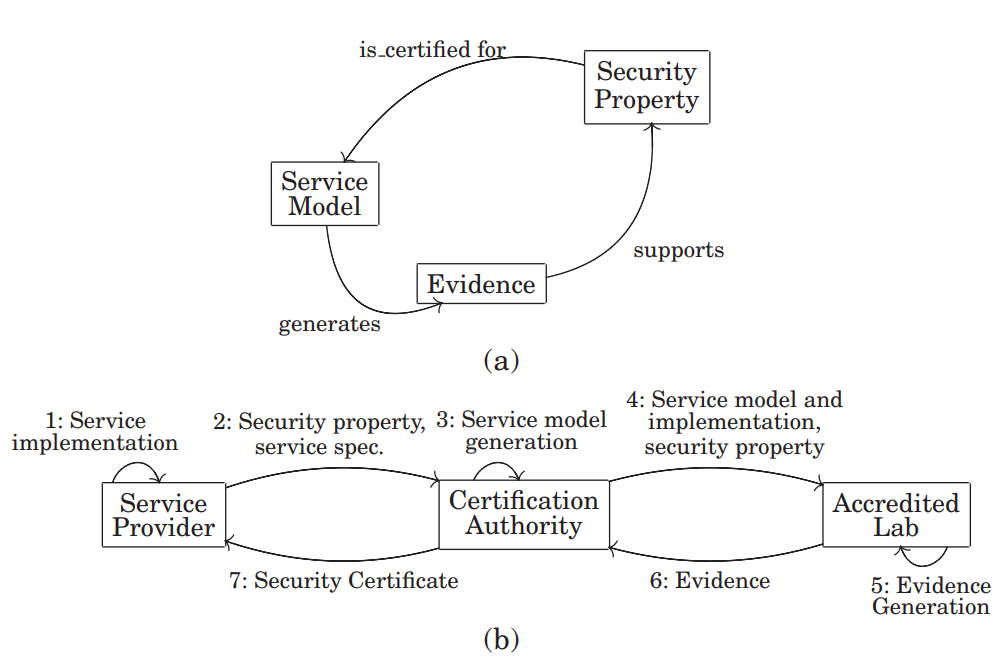
\includegraphics[width=\textwidth]{immagine_web_service.png}
\caption{Conceptual framework (a) and certification process steps (b) \cite{anisetti2013test}}
\label{Fig:OldProcess}
\end{figure}
\subsubsection{ITSEC}
ITSEC is a structured set of criteria with the scope of evaluating security within computer systems and products in the European Union; it was published in 1990 and was developed by France, Germany, Netherlands and UK governments, basing its features on the pre-existing, country-limited frameworks. This set of criteria was designed in the main part to be equally applicable to technical security measures in hardware, software and firmware products \cite{ITSEC}. ITSEC was centred around the Target of Evaluation (ToE) and assurance levels; these concepts made their way through all the versions of today's Common Criteria \cite{infrastructure2002common}.

\subsubsection{TCSEC}
TCSEC, commonly referred to as "The Orange Book" \cite{orangeBook}\cite{orangeBookDeath}, is a standard developed by the United States Government Department of Defense, and its scope was to evaluate and classify computer systems used for processing, storing and retrieving sensitive or classified information. This framework, like many others \cite{infrastructure2002common}\cite{ITSEC}, was developed around the following Evaluation Classes: 
\begin{itemize}
    \item D: Minimal Protection
    \item C1: Discretionary Security Protection
    \item C2: Controlled Access Protection
    \item B1: Labeled Security Protection
    \item B2: Structured Protection
    \item B3: Security Domains
    \item A1: Verified Design
    \item A2: Verified Implementation
\end{itemize}

\subsubsection{CTCPEC}
CTCPEC is a standard developed by the Canadian government with the same goals as ITSEC and TCSEC; in fact, it was a combination of the two. This approach finally led to combining the major standards and criteria into a single set: the Common Criteria \cite{CTCPEC}.

\subsubsection{Common Criteria}
\label{CC}
With these internationally approved standards, software companies finally had the tools to certify their products and sell them worldwide; however, every certification process had to be passed, resulting in a rather tedious and pricey process. Therefore, the Common Criteria (CC) was developed by unifying these pre-existing standards, following the approach of the CTCPEC, to allow companies to evaluate their products against a single set of standards. CC was developed by Canada, France, Germany, Netherlands, UK and USA governments and version 1.0 was issued in 1994; multiple agreements were signed in the following years to avoid useless re-evaluations and allow mutual recognition of CC certificates.
The Common Criteria for Information Technology Security Evaluation (also known as Common Criteria) represents the evolution of continuous and incremental certification schemes, and its latest versions are currently used to evaluate over two thousand major IT systems and applications (e.g. Microsoft Windows OS, McAfee anti-virus, Microsoft SQL Server \cite{CCProducts}).
CC is mainly based on the previous sets of standards' ideas:
\begin{itemize}
    \item Definition of the ToE, which includes the assignment of a Protection Profile, the description of the Security Target and the listing of the Security Functional Requirements.
    \item Definition of the Security Assurance Requirements
    \item Selection of the correct Evaluation Assurance Level
\end{itemize}

More details about the above phases are well described in \cite{infrastructure2002common}.

CC is now an established pillar in the security certification world, especially in the commercial industry, but it is not a perfect solution, especially when applied to highly dynamic systems like Edge and IoT. It is also worth noting that CC certifications are attributed to a specific version of the system under a specific configuration, and any configuration change or software update could mandate a re-certification process. To counter the redundancy of such processes, the CC designers proposed the Assurance Continuity (CCAC) re-evaluation process[], but the need to repeat the certification process is a big limitation. Therefore, the research never stopped; when considering highly dynamic domains such as those implied by the Cloud and Fog computing paradigms, it is important to define new certification schemes that better align with the context. 

%%%%%%%%%%%%%% da decidere se lasciarlo qui %%%%%%%%%%%%%%%%%%%%%%%%%


\subsection{Building Blocks of the Certification Schemes}
Modern certification frameworks rely upon several components defining how the process is executed and how the results should look. Below is a detailed list of the major pillars of certification frameworks with their fundamental functionalities as underlined by Anisetti et al. \cite{anisetti2017semi}\cite{anisetti2022multi}.

\subsubsection{Non-Functional Properties}
For the certification process of a system, it is important to establish some requirements that can be functional or non-functional preemptively, usually this is done during an initial risk assessment process. As stated by Chen et al. \cite{chen2013verification}: "broadly, functional requirements define what a system is supposed to do, and non-functional requirements define how a system is supposed to be", meaning that non-functional requirements focus on the system itself instead of what the system produces in output; once a requirement is proven to be satisfied by the system, it becomes a non-functional property of the same, and it can be expressed as follows: ⟨name, {(attribute, value), (attribute, value)}⟩. A property is composed of pairs "attribute-value" where the attributes are essential sub-properties that define the strength of the property. In other words, non-functional properties describe the system's capabilities and are usually grouped under the categories defined by the CIA triad: i) Confidentiality, ii) Integrity and iii) Availability. The CIA triad is an organizational model designed to guide information storing policies; its three parts are cybersecurity's three most crucial components. These properties are considered abstract because they represent generic security requirements and provide no information on how to achieve them. Instead, they are used to define concrete security properties. 

As defined by Anisetti et al. \cite{anisetti2013test}, a concrete security property is formally defined as follows:
A concrete security property, denoted \(p\), is a pair \( ( \hat{p}, A) \), where \(\hat{p}\) is an abstract property and \(A\) is a set of class attributes specifying the threats the service proves to counteract or the specific characteristics of the security function implemented by the service. 

The NIST defined these components as follows \cite{pub2005minimum}:
\begin{description}
    \item[Confidentiality] Preserving authorized restrictions on information access and disclosure, including means for protecting personal privacy and proprietary information. Confidentiality is a set of rules that limits access to information; ensuring confidentiality means the authorized entities can access the protected information and the unauthorized entities cannot. Confidentiality is accomplished through methods like data encryption and authentication procedures.
    \item[Integrity] Guarding against improper information modification or destruction, and includes ensuring information non-repudiation and authenticity. Integrity is the assurance that the information is trustworthy and accurate; it involves maintaining data consistency and accuracy over its entire lifecycle. For example, measures like file permissions and user access control ensure unauthorized entities cannot change data, while checksums and backups safeguard data from non-human threats like electromagnetic pulses or server crashes.
    \item[Availability] Ensuring timely and reliable access to and use of information. Availability guarantees reliable access to the information; it is best ensured by rigorously maintaining all hardware and staying up to date with all system upgrades; providing bandwidth, preventing bottlenecks and fast disaster recovery are also essential.

\end{description}



\subsubsection{Non-Functional Mechanisms}
For a non-functional property to be proven, a non-functional mechanism, in the form of \( ( name, \{ attribute, value \} )\), must be implemented to execute the certification process under specific configurations. Moreover, the property is what the process needs to verify, and the mechanism is the tool the system offers to test such property \cite{anisetti2017semi}; the verification is usually done through tests in the form of \\ \( (mechanism, (codde to execute, expected results))\). Finally, it is important to note that the mechanisms need to be described in the system's documentation; this allows the accredited laboratory to analyze and test them during the manual review phases.


\subsubsection{Target of Certification}
The application context and the system perimeter define the Target of the Certification (ToC); it describes the mechanisms on which the non-functional properties that need to be certified rely. Moreover, the evaluation of the certification scheme must verify the target’s (security) features. For example, in the Common Criteria process, the ToC (actually named Target of Evaluation) is accurately described in the Security Target Document.

\subsubsection{Evidence}
Evidence collection is the main step to proving that a given non-functional property is valid for a given ToC; it is important to note that evidence can be gathered by testing the service actively or passively. 
The property is finally assigned to the system when enough evidence is collected for a given requirement through well-aimed tests. 


\subsubsection{Life Cycle}
\begin{figure}[hb]
    \centering
    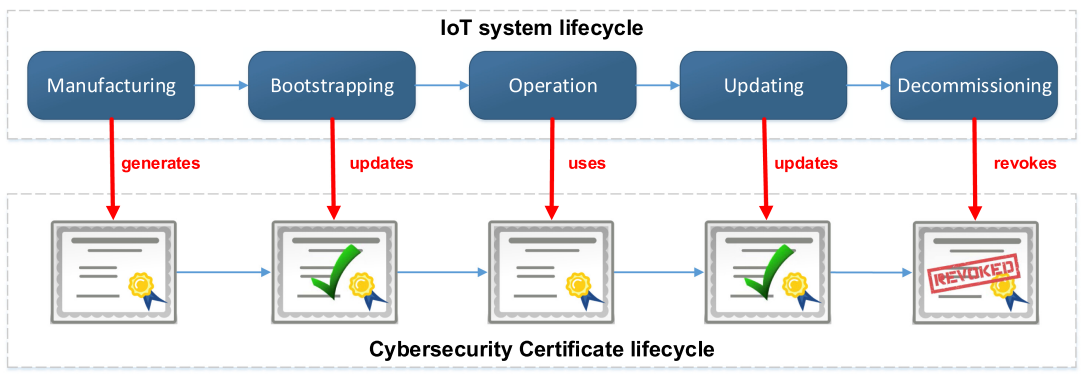
\includegraphics[scale=0.5]{images/lifeCycle.png}
    \caption{The cybersecurity certificate during the IoT device lifecycle.}
    \label{fig:lifecycle}
\end{figure}
As mentioned above, certificates are subject to invalidation, whether caused by a context change, a property change, or simply by the certificate's expiration; all certificates have a finite lifespan managed by the Certificate Authority (CA), which is usually also in charge of replacing it with a new one. However, the CA represents a bottleneck, and automation frameworks are needed when dealing with highly dynamic environments like Cloud and Edge. Therefore, the life cycle of a certificate is de facto a deterministic finite-state automaton whose state transitions are determined by specified conditions.

As mentioned above, certificates are subject to invalidation, whether caused by a context change, a property change, or simply by the certificate's expiration; all certificates have a finite lifespan managed by the Certificate Authority (CA), which is usually also in charge of replacing it with a new one. However, the CA represents a bottleneck, and automation frameworks are needed when dealing with highly dynamic environments like Cloud and Edge. Therefore, the life cycle of a certificate is de facto a deterministic finite-state automaton whose state transitions are determined by specified conditions. As shown in figure \ref{fig:lifecycle}, the lifecycle of a certificate is tightly coupled with the lifecycle of the IoT system, which is usually divided into five phases: i) Manufacturing, ii) Bootstrapping, iii) Operation, iv) Updating and v) Decommissioning. 

The manufacturing phase includes the production, programming and configuration of the system/device. This phase also includes the security certification process, which, if passed, assigns a brand new certificate to the system. The bootstrapping phase includes the installation and configuration of the device for the specific domain in which it will operate. Moreover, context-specific information should be embedded in the cybersecurity label (this step is too often ignored). It is also important to note that the context plays a fundamental role in every IoT system; a given device could require different security levels based on the type of information it needs to handle, and this variation can happen multiple times in the lifespan of the device. During the operation phase, the device/system provides its intended functionalities and should always be kept under a monitoring process. The monitoring is crucial to find new vulnerabilities and issues in the system. When a new vulnerability is found, and the manufacturer issues an update, rarely is a re-certification not issued due to the complexity of the analysis of the changes. Moreover, the security level and label are updated during a re-certification process. The decommissioning phase represents the end of the lifecycle of the system and includes the certificate revocation. This phase is also crucial because the devices composing the system could have stored sensitive information, and this phase's sole purpose is to make such information inaccessible \cite{surveyIOT}.

Typically, a certification process for Cloud services consists of a collaborative effort between four entities: i) a service provider who develops the service that needs to be certified, ii) a cloud provider supporting the service's certification, iii) a CA responsible for the definition of the requirements and the methodology and iv) an accredited lab to carry out the system evaluation. The problem of such an approach resides in the fact that continuous context changes can rapidly invalidate the assigned certificates, and without proper context testing techniques, it is necessary to re-certificate the whole service every time. The framework that M. Anisetti et al. proposed addressed this issue by constantly verifying the possessed certifications against the context changes to prevent unnecessary revocations and re-certifications.


\subsubsection{Labels}
Labelling schemes exist to straightforwardly inform the user about the security certification that has been executed on a device; such schemes should contain the following main groups of information:

\begin{itemize}
    \item Domain that was considered while performing the certification activity; the certification should be revoked the moment the device leaves it

    \item Level of assurance; states the security tests performed to certify the device. Usually, the level of assurance is associated with the protection profile of the specific domain

    \item  Information about the achievement of the certification, such as the responsible entity, the process and the validity period

\end{itemize}

Even though the importance of labels is mostly tied to commercial purposes \cite{baldini2016security}, perhaps, they could also be read by the Certification Authorities to have a quicker overview of the system's mechanisms and capabilities. In state-of-the-art schemes, labels are ignored or poorly used, but they might play a fundamental role in future schemes.


\subsection{Assurance for Highly Distributed Paradigms}
As described in section \ref{Edge}, Edge computing adds multiple challenges to the table in terms of functionalities, especially when combined with IoT layers, which bring on even more security and assurance topics. Mahmud et al. \cite{mahmud2018fog} highlighted three security aspects that will inherently haunt new highly distributed computing paradigms:
\begin{itemize}

\item Technological discoveries advance at different paces for software and hardware; new software architectures (like edge computing) are designed upon traditional components, especially for networking, raising the number of vulnerabilities to attacks.

\item Highly distributed systems make it difficult to ensure secure authentication and privacy in every node at all times; monitoring frameworks could be insufficient in many cases.

\item Security mechanisms for data-centric integrity can greatly affect the quality of service of these systems.

\end{itemize}



%%%%%%%%%%%%%%%%%%%%%%%%%%%%%%%%%%%%%%%%%%%%%%%%%%%%%%%%%%%%%%%%%%%%%

\subsection{New Certification Efforts in Cloud Environments}
Cloud service certification has been a highly focused research point in recent years and is now considered a mature assurance feature. Moreover, as identified by M. Anisetti et al. in \cite{anisetti2017semi}: "Compared to traditional service certification, cloud certification is: i) highly dynamic, it is affected by contextual changes at any layer of the cloud stack, ii) multi-layer, it can refer to services at different cloud layers; iii) intrinsically incremental, it requires continuous validity verification and incremental adaptation with the scope to minimize costly re-certification activities, and iv) trustworthy by delegation, it requires advanced trust models based on delegation to support cloud peculiarities". M. Anisetti et al. also proposed a continuous and incremental approach to Cloud service certification, providing a formal description of the audit-related evidence collection. Such an approach is founded on five main pillars: non-functional properties, non-functional mechanisms, Target of Certification (ToC), evidence collection and the life cycle of the certification. The proposed certification process can be simplified with the following steps: i) Non-functional properties definition, ii) ToC definition, which includes the description of the non-functional mechanisms offered by the system, iii) Tests definition, iv) Tests execution, which involves evidence collection and analysis and v) Certificate release.


This process involves different entities, such as the service provider, the cloud provider, the certification authority and an accredited laboratory; this way, a chain of trust is formed, and the responsibilities are evenly spread between the entities involved. It is also split into an issuing phase, where the process is responsible for all the evaluation activities, and a post-issuing phase, which continuously verifies the certificate's validity against eventual context changes \cite{anisetti2017semi}.

\subsection{New Certification Efforts in Edge Environments}
Certification schemes over Fog/Edge computing nodes are a recent and less mature topic; when dealing with a network composed of countless devices (the Fog nodes), it is fundamental to have a completely automated framework capable of handling the whole certification process for each node. The scheme proposed by Aslam et al. in \cite{aslam2020fonac} addressed the matter with automated and continuous monitoring and auditing of the Fog nodes; nevertheless, this total automation relies entirely on the backend provided by the Cloud infrastructure that acts as an inner CA for its Fog layer, inheriting all its vulnerabilities. The differences between this approach and the ones proposed for the Cloud are the requirements for the certifications. Fog nodes have limited functionalities and need to be quickly admitted to the Fog layer; meanwhile, there is a need to execute much stronger certification activities on the Cloud stack.

\subsection{Current IoT Certification Efforts}
Internet of Things is not a new concept, and so is not the need for dedicated certification schemes; The rapid spread of systems relying on IoT highlighted many limitations of the most known certification schemes.

\subsubsection{Common Criteria}
As described in section \ref{CC}, CC is the most used on every type of system (Cloud, Edge, IoT) thanks to its Mutual Recognition Agreements (MRA) and to the depth the certification process can reach. However, the industry and the research community have underlined three major limitations that make it hardly applicable in the IoT world \cite{kaluvuri2014quantitative}\cite{keblawi2006applying}:
\begin{enumerate}
    \item It takes too much time and effort, resulting in a slowdown of the system and the risk of overwhelming the single devices with testing requests.
    \item Systems classified with high EALs are attributed to highly complex documentation, making the comparison with other certificates difficult, hence, not complying with the harmonization challenge (more about this in the commercial section).
    \item Managing changes is almost non-existent, even with the CCAC version, limiting the number of updates the manufacturer can issue and drastically reducing system operativity during re-certification.
\end{enumerate}


\subsubsection{ICSA Labs IoT Security Testing Framework}
A newer framework is the one proposed by the ICSA Labs company. The ICSA Labs IoT Security Testing Framework is focused on IoT systems, more specifically, on the security of the single devices participating in an IoT environment. The approach is based on a periodic assessment and update of the certification criteria, and it includes frequent iterative updates, addressing the dynamic environment challenges and the evolving cybersecurity threats inherent to the IoT paradigm. This process is more focused on the iterativity of the assessments and less on the depth of the certification, leaving aspects such as the labelling ignored \cite{ICSAFw}.

CC remains the most used and studied certification scheme, while others like Commercial Product Assurance, Cybersecurity Assurance Program and the Certification de Sécurité de Premier Niveau fall into a commercial and country-specific side.


\subsubsection{Industrial And Commercial Purpose Schemes}
From the commercial and industrial point of view, several challenges have been highlighted in the definition and deployment of an IoT security certification framework; some of these are not part of this thesis' focus but are still relevant for a complete overview of what a certification framework should guarantee at a certain point; furthermore, table \ref{Tab:comparison} shows a quick comparison of the approaches discussed below.
\begin{enumerate}
    \item Standardization: Since the IoT landscape is still fragmented in approaches and standards, it is crucial to start aligning the efforts for a more homogeneous perspective.


    \item Harmonization: while there is the need to align the standards, there is also the need to allow different ones to coexist and be mutually accepted.


    \item Time, complexity and cost: Manual processes, direct testing and complex documentation guidelines of currently available approaches are heavy on resources like time and money, and the need to minimize this weight is crucial for a for-profit company, especially with IoT systems that need frequent re-certifications.


    \item Dynamic environment: IoT systems are often deployed in dynamic environments whose conditions might affect the security level of a device. Moreover, a device should be able to receive an update and change its or the system's configuration without invalidating the certificate completely.


    \item Influence of the context: The context in which an IoT system is deployed is not ignorable; indeed, it determines many of the security features the system will require. Moreover, the context and the system's purpose should be linked to determine the sensitivity of the managed data.


    \item Transparency to the end-user: A company must help the clients understand the positive aspects of the system's certification, especially when different approaches are not directly comparable. For this purpose, it is becoming a common rule to attribute security labels to the certificated devices; such labels should clearly and concisely represent the value of the certification's level. Labels' goal is ultimately to allow users to easily compare different levels of frameworks without knowing the approaches' details.


    \item Support for the certificate lifecycle: cybersecurity certificates carry validity periods that regulate and confirm the authenticity of the involved entities. It is important to ensure that the certification is supported and updated during its lifecycle and that all the certificated properties remain valid during this period.

\end{enumerate}


It should be noted that apart from the AC version of Common Criteria, no other approach considers a lighter process for re-certification processes.

Some available frameworks are adopted more frequently than others; in the following section, the most known and used in the industry will be presented and compared to highlight the major weaknesses that should be considered when developing new certification schemes \cite{surveyIOT}.

\subsubsection{Commercial Product Assurance}
The Commercial Product Assurance (CPA) is a certification scheme developed by the UK Communications-Electronics Security Group (CESG) for national public purposes. CPA allows only security-related patches and updates, and thanks to its "lightweight" design, it drastically reduced the re-certification process length; however, it is not enough. The average re-certification still takes at least six months to complete, reducing the system operativity during this time.

\subsubsection{Cybersecurity Assurance Program}
Cybersecurity Assurance Program (CAP) is a certification methodology developed by the Underwriters Laboratories company (UL) that adheres to their proprietary UL 2900 standards. Unfortunately, being a private and for-profit organization drastically reduces the community's trust in its certificates since they are not provable by third-party experts and do not adhere to the standardization and harmonization challenges.

\subsubsection{Certification de Sécurité de Premier Niveau}
The National Cybersecurity Agency of France developed certification de Sécurité de Premier Niveau (CSPN) in 2008 to verify the products' compliance with their security specifications in a timely manner. Unfortunately, this certification framework is standardized in France but not officially recognized by any other country, making it useless for international products.

%%%%%%%%%%%%%%%%%%%%%%%%%%%%%%%%%%%%%%%%%%%%%%%%%%%%%%%%%%%%%%%%%%%%%%%%%%%%%%%%%%

    


\begin{table}[htb]
    \centering
    \begin{tabular}{ |p{3cm}|p{2.3cm}|p{2cm}|p{2cm}|p{2cm}|p{2cm}|  }
         \hline
         \textbf{Challenges}&\textbf{CC}&\textbf{CPA}&\textbf{CAP}&\textbf{CSPN}&\textbf{ICSA Labs}\\
         \hline
         \textbf{Certification time (months)}* & 4-9 EAL2, 6-12 EAL3, 9-24 EAL4.
         & 6-18 & 6+ & 1-2 & 1-2\\
         \hline
         \textbf{Documentation} & Higher the EAL more complex the documentation & Hard to compare & Hard to compare & Hard to compare & Hard to compare\\
         \hline
         \textbf{Changes management} & Certificate valid only for specific patch and configuration & Any change is manually reviewed and can invalidate the certificate & Any change is manually reviewed and can invalidate the certificate & security patches invalidate the certificate & Any change is manually reviewed and can invalidate the certificate\\
         \hline
         \textbf{Context consideration} & \cmark & \xmark & Partially & \cmark & \cmark \\
         \hline
         \textbf{Monitoring} & \cmark & \cmark & \cmark & \xmark & \cmark \\
         \hline
         \textbf{Validity period} & Variable & Variable & 1 Year & 8 Weeks & 1 Year \\
         \hline
         \textbf{Labels completeness} & Only EAL info & \xmark & \xmark & \xmark & \xmark \\
         \hline
         \textbf{Mutual Recognition Agreements (MRA)} & Accepted by numerous countries & UK only & Not standard & France only & Not standard \\
         \hline
         \textbf{Cost (\$)}* & 75-200k EAL2, 110-250k EAL3, 150-350k EAL4 & 1300 per work day & Not standard & 25-30k & Not standard \\
         \hline
         \hline
         \multicolumn{6}{| c |}{\em*GAO analysis of data provided by laboratories.}\\
         \hline
    \end{tabular}
    \caption{Commercial Purpose Schemes Comparison}
    \label{Tab:comparison}
\end{table}


%%%%%%%%%%%%%%%%%%%%%%%%%%%%%%%%%%%%%%%%%%%%%%%%%%%%%%%%%%%%%%%%%%%%%%%%%%%%%%%%%%






\section{Configuration Changes}
A configuration change refers to modifying a component subject to change control. For example, some configuration changes that might interest an IoT system are the relocation of an asset (e.g. device, edge node, cloud server) or the change of some security property's attribute values.
Fields and attributes designated for change control are referred to as configuration information. There exist three main types of configuration change control \cite{IBMConfChange}:
\begin{description}
    \item[Configuration Change Tracking] Changes are tracked in the component record and automatically applied to the target attributes. This type of control can be paired with the other ones.
    \item[Revision Tracking] Based on revision versions that are incremented every time an update occurs. The revision records are used to support the configuration change tracking, which has to be present. This approach can also be combined with the approval-based change control, but when it is not, it is possible to change the configuration element directly in the component record.
    \item[Approval-Based Change Control] Configuration information cannot be altered without engineering change approval when this control change approach is involved. The evaluation involves using change or revision records to plan, approve and execute configuration changes; the used record is considered the engineering change record during this phase and provides core information about the history of past changes. Given the need for a configuration record, this approach can be combined with any other one.
\end{description}

Configuration changes represent a critical point in the cybersecurity certification frameworks because a certificate cannot predict how a system will be affected after one. Moreover, even though most developers are focusing on creating software that should not need a system restart after an update, the results are weak, and the system downtime represents another critical aspect for IoT systems. It should also be noted that an IoT system update includes the transferral of updated data and programs to all the devices composing it, resulting in a rather long downtime, depending on the system's topology and resources. Furthermore, downtime represents an issue for certification frameworks, especially for this thesis' proposed solution, due to the inability to start an evaluation process on the system.
To address the downtime matter, M. Ciok et al. recently proposed a platform to help developers with the system's architecture \cite{mateusz2022flex}.




\section{Looking Forward}
Certification schemes went a long way and passed through many iterations of improvements, optimizations and agreements; now, it is clear that no approach is perfect, especially when dealing with new generation systems that often include IoT layers in their stack. In addition, the IoT paradigm is much more dynamic than the cloud, both in the software and hardware, resulting in remarkably higher costs in terms of time and money; for this reason, the classic approaches seem not to be feasible anymore and result in being too restrictive for the IoT system manufacturers. The ideal certification scheme should be less rigorous in terms of assumptions and remove most costs (the manual phases). Such a scheme should deal with more variables, like unknown mechanisms, properties and attributes; a quick, ephemeral certification scheme that would verify only the strictly needed properties with the minimum effort to allow the system to keep operating right after remote configuration or context changes. Such an ideal scheme should address the following challenges:
\begin{enumerate}
    \item How should the properties be modelled now?\\ 
    As discussed in this chapter, current schemes rely on properties that are not expected to change, and their changes can lead to expensive, slow and redundant recertifications; finding new models for the system's properties is essential to allow manufacturers to keep updated their systems.
    
    \item Which of the other certification building blocks should change, and how?\\
    If the properties' model change, it is crucial to identify which of the other building blocks would be affected and which could be optimized.
    
    \item Remembering that some mechanisms might not be known, given a system and a property, what steps should be included in the new certification process to certify such property of the system?\\
    Non-functional mechanisms are usually known at certification time; this allows the laboratories to execute well-aimed tests to demonstrate the properties of the system exploiting such mechanisms. However, when dealing with dynamic systems, some configuration change could add or disable a mechanism which could not be easily detected; hence, it is important to design a scheme capable of dealing with this issue.
    
    \item How should the process deal with the limited resources of an IoT device/system in the testing phase?\\
    Downtime is another IoT system's major issue when dealing with recertifications. Some systems cannot afford to be disabled for long periods, but IoT devices have very limited resources. Minimizing the load and resorting to new testing methods could be needed to overcome this issue.
\end{enumerate}

The next chapter will focus on making the first step toward a new recertification scheme to address such challenges, specifically, challenges 1,2 and 4. It will introduce the scoring system and the trigger component that will make the process as fast and automated as possible; moreover, properties, attributes, evidence collection and certification will be remodelled and deeply discussed. Finally, the new models are introduced to obtain an extremely lightweight scheme that will allow manufacturers to recertify their systems with the minimum possible effort quickly.




\chapter{Methodology}
\label{cap3}

Chapter \ref{cap2} shows that previous iterations of certification frameworks dealt with non-functional properties, attributes and mechanisms, assuming to know them when needed. This approach was valid in Cloud environments because all the required properties to be certified were manually pre-established and specified during a preparation phase before the certification execution. However, the process implied a rather large overhead when certifying a whole new system or issuing a recertification process after a small configuration change. In Cloud environments, a slow process is acceptable due to the small number of changes a Cloud system usually has to go through and the high accuracy requirements. On the other hand, IoT environments are highly dynamic, unique and continuously subject to small configuration and patch changes making this approach no longer feasible due to the high overhead each certification process would introduce and the resource cost, especially in the manual preparation phase.

As described in chapter \ref{cap2}, a certification process is usually made of four main steps: i) definition of the non-functional properties ii) definition of the certification target and of the mechanisms that will allow testing a given property iii) tests definition, aimed at collecting evidence proving the property iv) tests execution and evidence collection. So, for example, a test to collect evidence over the attribute \(x\) would be a pair \( (M_x, (c, R_e) ) \) where \(M_x\) is the mechanism the system offers to test the attribute \(x\), c is the code to execute, and \(R_e\) is the expected result of the test code execution; if the concrete results are close enough to the expected ones, the certificate can be released.

The main issue of directly transferring such a process over IoT systems is the resources and time required to complete it, especially because there is almost no difference between a full certification and a recertification process in state-of-the-art techniques. Assuming that a brand new IoT system should undergo a full certification process, finding a lightweight and less strict solution is necessary to reduce the unease caused by recertification processes since their goal should only be to maintain most of the ``strength" the original certificate already possessed. Another variable such solution should deal with is the ``quantity" of changes the system went through before triggering the recertification process; combined with the wide variety of contexts and devices that an IoT system may be involved with, it makes it crucial to generalize the process.

A way to generalize a certification process whose main objective is to be fast and lightweight, even though sacrificing some accuracy, is to remove the assumption of knowing a priori all the properties, their attributes and the mechanisms the system offers to test them. By removing the majority of the manual preparation phase, properties information will have to be extracted dynamically at execution time using evidence extraction techniques in a ``discovery" phase, aiming to uncover some properties and their values from the certification target to classify and evaluate them. Furthermore, the high dynamicity of IoT systems implies continuous and unpredictable state transitions that inevitably involve the transformation of various attribute values. Such changes make it essential to not only define thresholds to validate attributes and properties but also ranges some of those values can shift within.

The recertification process is triggered when specific security conditions are met after a system undergoes a configuration change; the components of such process need to adapt to the new approach, and for the current step this thesis is taking, their models inevitably need to change. Therefore, this chapter introduces all the required components: i) attributes, ii) properties, iii) trigger, and iv) tests and evidence collection models. In addition, the scoring system guides the certification process, allowing one to express how strong the certificate should be. Moreover, properties and attributes are still at the basis of the proposed certification scheme, but properties are now referred to as micro-properties, each of whom is categorized under a specific macro-property; such separation grants a wider grade of control over the scoring system. Furthermore, the trigger is a new component whose task is to send an alert whenever a configuration change alters one or more security properties, detailing all the needed information about such properties and the involved attributes. Finally, the evidence collection model is built around the other components' models and allows specifying detailed information about the testing phase that must be executed. The interaction between such components and the general flow of the proposed process is shown in figure \ref{fig:comps}.



\begin{figure}[ht]
    \centering
    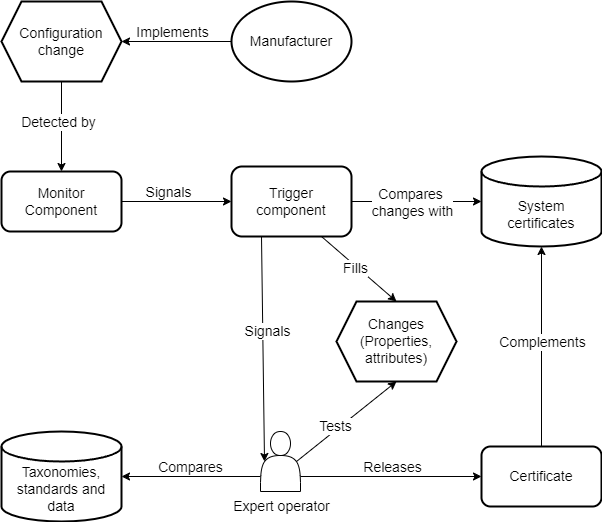
\includegraphics[scale=0.7]{images/components.png}
    \caption{Proposed scheme's components and interactions}
    \label{fig:comps}
\end{figure}


\section{A Simple Example Scenario}
\label{scenario}
Given the above overview of the main components of the proposed certification scheme, it is useful to keep in mind a simple example scenario that will support the further explanation of the components in the following sections.
This section illustrates a simple contextual example to improve the visualization the proposed idea; we note that many details of this example are further developed in the following sections. This example scenario shows how a specific situation could be handled using the proposed scheme and will be used as a reference in the next sections.

Let us consider a smart city environment where the manufacturer needs to add security cameras. Since the contract with the system's owner requires a certificate that any produced data is secured, the system needs a quick re-validation to prove that the recorded images are indeed securely stored. This scenario could involve many properties, however, only two of them and one attribute for each property will be considered in this example for simplicity: referring to the properties taxonomy in appendix \ref{taxonomy}, let us consider the portion related to secure storage, which includes the following properties and attributes:

\begin{description}
    \item[\(p_1\)] The ability to support data encryption at rest (encrypt passwords, device id and other authentication data) and the considered attribute is the following. Assuming that the encryption algorithm is AES \cite{daemen1999aes}, the property can be refined in terms of attributes (\ref{bblocks}) specifying the length of the key, that is, i) 128 bits, ii) 192 bits, or iii) 256 bits.
    
    \item[\(p_2\)] The ability to ``sanitize" or ``purge" specific or all data in the device and the considered attribute is the followingn: given that the storage eraser algorithm is the U.S. Department of Defense (DoD) 5220.22-M algorithm \cite{fischer2017dod}, an attribute can be the number of times the data is overwritten, and the value can be 3 or 7.
\end{description}


In the remainder of the chapter, we show how this scenario could be handled in a rather quick and less costly way using the proposed scheme as opposed to the traditional ones. The next sections introduce and formalize the components representing a step toward our goal, and the aspects of the just presented scenario are developed along the chapter, demonstrating how each can be adapted to the new challenges brought up by the new highly dynamic systems (IoT).


\section{The scoring system}
Before introducing the main components of the certification scheme, it is important to present the concept of score and how the scoring system works; a score is assigned to each attribute based on its value and the purpose and context of the entire system. The score of a property is then calculated by summing the scores of its attributes. Finally, the weighted sum of all the properties scores determines the certificate's strength; additionally, for the certificate to be valid, such a total must reach a pre-determined threshold. Expert manual operators should decide the score values and the thresholds with the help of taxonomies, standards and knowledge.

\begin{example}
\label{xmp:1}
Following the example scenario in section \ref{scenario}, the ranges of scores assigned to the attributes could be [10, \dots, 70] for the AES algorithm attribute and [40, \dots, 80] for the U.S. DoD 5220.22-M algorithm.
Since the sum of the properties scores finally defines the certificate's strength, such a sum must reach at least the defined threshold, which could be set at 100 with a weight of 1, for example.
\end{example}


\section{Attributes}
As for the state-of-the-art approaches, properties will still be modelled using attributes that define them at a lower level; more specifically, in the proposed approach, attributes define micro-properties, and are defined in a slightly different way from state-of-the-art schemes. 

\begin{defn}
An attribute \(a\) is defined as a pair \((\hat{a}, [value_{min}, value_{max}])\) where \(\hat{a}\) is the abstract attribute and \(value_{i}\) is a possible value of \(a\). 
\end{defn}

In other words, an attribute is now defined by its name and the list of values it can assume. We note that the range of possible values is considered sorted by relevance, from the less relevant to the most relevant. For example, the value of the response time of a device is more relevant the lower it is; contrary, the value of a storage size is more relevant the bigger it is.

The score range of an attribute should be decided by an expert person having knowledge of the system and the context; such range should be balanced, setting the lowest score corresponding to the lowest relevant valid value and vice-versa.
The linear mapping (mapping that maintains a constant ratio between points) operation in the equation \ref{eqn:mapping} allows mapping values between two ranges, in this case, values and scores.

\begin{equation}
\label{eqn:mapping}
    q = \left \{ (p - A) \times \frac{D - C}{B - A} + C \bigm| [A, B] \in \mathbb{N} \wedge [C, D] \in \mathbb{N}  \right \}
\end{equation}

Considering the range of valid attribute values from A to B, the range of scores from C to D, and the actual attribute value p, the mapping allows computation of the corresponding score value q.
A linear mapping requires two operations: a scaling operation to make the ranges the same size and an offset operation to align the ranges. Since scaling is always relative to the origin, the first step is to shift the range [A, B] to the origin by subtracting A from p; next, scale p by the ratio of the range sizes (D-C)/(B-A). Finally, shift this value to the start of the [C, D] range by adding C, resulting in the equation \ref{eqn:mapping}. By rearranging the terms of the equation, it is possible to extract the scale and offset factors that compose it:

\[scale = \frac{D - C }{B - A}\]
\[offset = -A \times \frac{D - C}{B - A} + C\]
\[q = \left ( p \times scale \right ) + offset\]


This equation maps the attribute's values range to the scores range spreading the values evenly (e.g., “equal importance” expressed with W[0] = 1/n, W[1] = 1/n, \dots , W[n]= 1/n). If the attribute's values are not numerical, they should be pre-emptively mapped to a list of indices; the indices list should then be used instead of the attribute's values. If the obtained value is not a whole number, the result should be ceiled to next whole digit. Finally, the result should be rounded up in case it does not exactly match a value because rounding down would result in a weaker-than-expected certificate. For example, for the micro-property Interface Control (ref), it is necessary to have a list of supported communication technologies that could include IEEE 802.11, Bluetooth and Ethernet connections; such a list might be mapped with an index list [1,2,3] where 1 refers to IEEE 802.11, 2 to Bluetooth and 3 to Ethernet.


\begin{example}
Following Example \ref{xmp:1}, equation \ref{eqn:mapping} can be used to determine which values will be tested for each attribute. First, a couple of steps need to be done: i) substitute the lists of values with lists of indices; [1,2,3] for the AES algorithm attribute (\(q_1\)) and [1,2] for the U.S. DoD 5220.22-M algorithm attribute (\(q_2\)), and ii) the threshold of 100 should be evenly distributed across the score ranges to determine the score each attribute should obtain, namely, T/n where T is the threshold (100) and n is the total number of attributes (2). Then, the values can be discovered using the equation:
\begin{align*}
  q_1 = (50 - 10) \times \frac{3 - 1}{70 - 10} + 1\\
  q_1 = 40 \times \frac{2}{60} + 1 \\
  \llap{$\rightarrow$\hspace{50pt}} q_1 = \Bigl\lceil\frac{7}{3}\Bigr\rceil = 3
\end{align*}
\begin{align*}
  q_2 = (50 - 40) \times \frac{2 - 1}{80 - 40} + 1\\
  q_2 = 10 \times \frac{1}{40} + 1 \\
  \llap{$\rightarrow$\hspace{50pt}} q_2 = \Bigl\lceil\frac{5}{4}\Bigr\rceil = 2
\end{align*}

When translating back the indices to the real values, the results show that to reach at least the set threshold of 100, attribute \(q_1\) needs to have a value of 256 bits and attribute \(q_2\) needs to have a value of 7.
\end{example}

The mapping also allows the system to compute the minimum values that each attribute of each micro-property needs to have to release a certificate with the minimum effort. Such values should then be gathered with a simple getter function.

\[ComputeMinValues([a_1, \dots , a_n], threshold)\]
\[GetMinValue(a_j) \rightarrow {value_a}_j\]

Where \textit{ComputeMinValues} invokes the Equation \ref{eqn:mapping} and stores the results for each attribute, and \textit{GetMinValue(\(a_j\))} returns the value that needs to be tested for the attribute \(a_j\).

\section{Properties}
The traditional definition of functional-property (e.g. in \ref{bblocks}) is now referred to as micro-properties, and they have been organized into three categories referred to as macro-properties.
\begin{defn}
A micro-property p is a pair \(\langle \hat{p}, \left \{  (a_1, value_1), \dots , (a_n, value_n)\right \} \rangle\) 
where \(\hat{p}\) is the abstract micro-property and \(\left ( a_i ,value_i \right )\) is a pair representing an attribute of the property and its value.
\end{defn}

In other words, micro-properties are defined by their attributes and the corresponding values.


On the other hand, macro-properties are intended to group micro-properties that influence similar aspects of the system; more specifically, every micro-property contributes to one of the macro-properties, namely, \textit{Confidentiality}, \textit{Integrity} and \textit{Availability}. Macro-properties have a specific function in the proposed approach, helping with the micro-properties score attribution; since the thresholds will be based on the macro-properties, every micro-property's score will influence its macro-property final weighted score.

\begin{defn}
A macro-property of the system P is defined as a triple \\ \( \Bigl\langle \hat{P}, \left \{(p_1, score), \dots , (p_n, score )\right \}, wscore \Bigr\rangle \) where \(\hat{P}\) is the abstract macro-property, \( \left (p_i, score \right ) \) is a pair representing a micro-property and its score, and \textit{wscore} is the total weighted score of the macro-property; the weight determining the final result should depend on the context.
\end{defn}

By way of explanation, macro-properties act as abstract containers of micro-properties and scores, allowing for better control over which categories of micro-properties should be prioritized during a certification process.

\begin{example}
Following the example in Section \ref{scenario}, the properties described translate directly into micro-properties, which are then categorized under the Confidentiality macro-property. The resulting model is:
\[ \Bigl\langle Confidentiality, \left \{(p_1, 70), (p_2, 80)\right \}, 150 \Bigr\rangle \]
Where:
\begin{itemize}
    \item \(p_1 = \langle \hat{p_1}, (q_1, 256)\rangle\)
    \item \(p_2 = \langle \hat{p_2}, (q_2, 7)\rangle\) 
\end{itemize}

\end{example}

\section{Trigger}
\label{trigger}
The trigger is a component detecting security changes in the system, evaluating them and acting in case these changes should impact crucial security properties. The trigger should also have continuous access to the system's information and certificates to detect changes accurately. The framework should access such changes through the \textit{Changes} function. 

\begin{defn}
The \textit{Changes} function is defined as \(Changes() \rightarrow \left \{ \left ( p_j, \left \{ a_k \right \} \right ) \right \} \), where \(p_j\) is a micro-property of the system and \( \left \{a_k \right \} \) is the set of specific attributes changed or added by the update.
\end{defn}

Such a function includes multiple background operations that the system has to deal with; these functionalities should probably include a monitoring framework for change detection. The monitoring should be invoked automatically every time a system (or context) update occurs. It should then compare the updated changes with the security properties and their attributes; any change over a security property should be immediately added to the \textit{Changes} function output list. We note that this low-level implementation details are out of the scope of the current thesis, and function Changes abstract these details into a uniform interface. Moreover, the trigger component should also be notified about the availability of new changes.


\section{Evidence Collection Model}
\label{evmodel}
Evidence collection is the process that, given a system and a property, gathers evidence proving the system holds such property through a series of tests.

\begin{defn}
    A test \textit{t} is modelled as a pair \( \langle \hat{p}, \left (a_j, value_j, c_j \right ) \rangle \) where
    \begin{itemize}
        \item \( \hat{p} \) is the micro-property to test;
        \item \(a_j\) is an attribute of the micro-property;
        \item \(value_j\) is the expected value of the attribute;
        \item \(c_j\) is the code to execute to gather evidence over the attribute \(a_j\);
    \end{itemize}
\end{defn}

In other words, each test case is specifically aimed at demonstrating that a system's attribute holds for a specific value; once all the attributes included by a micro-property have been demonstrated, the micro-property can also be considered demonstrated.
Additionally, the set of all tests form the evidence collection model, as follows.

\begin{defn}
The evidence collection model \(\mathcal{E}\) is defined as a set of elements, one for each micro-property, and it is modelled as \(  \left \{ \left \{ t_j \right \} {_{\hat{p}_i}} \right \} {_{\hat{P}_j}} \) where \( \hat{P}_j \) is a macro-property, \( \hat{p}_i \) is a micro-property, and \(t_j\) is the test to evaluate the attribute \textit{j} (\(a_j\)).
\end{defn}

In other words, the evidence collection model E is a list of test cases where each test aims at verifying that an attribute holds a specific value. The gathered evidence is then eventually stored in the released certificate.

\begin{example}
Following the previous examples over the scenario introduced in Section \ref{scenario}, the tests can be represented as follows: 
\begin{itemize}
    \item \(t_1 = \langle p_1, (q_1, 256, c_1) \rangle\)
    \item \(t_2 = \langle p_2, (q_2, 7, c_2) \rangle\)
\end{itemize}
Given such tests definitions, it is possible to express the evidence collection model: 
\[\{\{t_1\}_{p_1}, \{t_2\}_{p_2}\}_{Confidentiality}\]

\end{example}

\section{Certification Model Definition}
Once the trigger component starts the process by providing the system changes information, an important component that needs to be used for the recertification is the set of old certificates \(\mathcal{C} = \{c_1, \dots, c_n\}\); they contain all the demonstrated properties with their score and collected evidence prior to the update. Therefore, the proposed scheme is expected to provide a function \textit{Ephemeral} to obtain the certification model for the updated system. We note that the \textit{Ephemeral} function resumes the majority of the tasks of the scheme; this was introduced to simplify the mean of explanation.

\begin{defn}
The \textit{Ephemeral} function is defined as \(Ephemeral(\mathcal{C}, system_{t+1}) \rightarrow {\mathcal{M}}_{t+1} \), where 
\(\mathcal{C}\) is the set of certificates released for the system up to the time \textit{t}, \textit{t+1} represents the time after the update, and \(\mathcal{M}_{t+1}\) is the certification model for the updated system.
\end{defn}

The Ephemeral function returns the certification model needed for the certification process. Moreover, the certification model details all the activities required to certify a given target against the macro-properties affected by the configuration change. Once the new certification model is computed, it will be possible to call the \textit{Execute} function that will execute the tests on the system based on the given certification model returning the new certificate if all the requirements are satisfied. 

\begin{defn}
The certification model is defined as 
\(\mathcal{M} = \left ( \left ( P_1, P_2, P_3 \right ), \mathcal{E} \right )\) where \(P_i\) is a macro-property and \( \mathcal{E} \) is the evidence collection model.
\end{defn}
Namely, the macro-properties that compose the certification model \(\mathcal{M}\) are:
\begin{itemize}
    \item \(P_1\) is the Confidentiality macro-property
    \item \(P_2\) is the Integrity macro-property
    \item \(P_3\) is the Availability macro-property
\end{itemize}
 
The framework should then be able to call the \textit{Execute} function using the certification model to deliver a new ephemeral certificate. Such certification model is computed at the begining of the process and it is bound to the target system.The execute function allows obtaining the new certificate for the updated system and automatically adds it to the set of system's certificates \(\mathcal{C}\).

 \begin{defn}
 Each certificate is then defined as a set of pairs \( (p, \{e_j\}) \), where \(p\) is a micro-property with the set of evidence supporting it \( (\{e_j\}) \).
 \end{defn}
 
\begin{defn}
The \textit{Execute} function is defined as \( Execute(\mathcal{M}_{t+1}) \rightarrow \mathcal{C} \cup \{c_{t+1}\} \), where \( \mathcal{C} = {c_0, \dots , c_t} \) and \(c_i\) is the certificate released at time \(i\).
\end{defn}
 

 
 The system will finally be attributed a new certificate that will complement all the previously obtained ones and will carry all the information of the re-certification process that occurred after the update, including tested micro-properties and attributes, tests information and gathered evidence.



\section{Discussion}

For the next chapters, it is essential to clarify all  the major assumptions made during the design phase of the proposed certification process. As described in chapter \ref{cap2}, the current efforts in the IoT world are directed toward highly distributed systems (Edge computing) that involve some central computing nodes (Cloud computing). Therefore, when referring to IoT systems in the next chapters, it will be implied that the system will be composed of a Cloud layer, an Edge layer and an IoT layer. We note that the ToC model defined in chapter \ref{cap2} is still valid and has not been considered in this thesis work for simplicity, although in future, it could be modelled differently to better suit the new frameworks. Furthermore, it should be noted that this thesis' focus is on maintaining the certification's validity during the system's life cycle, mainly after some configuration change. Hence, when dealing with examples in the future chapters, it will be assumed that every system has already been fully certified with a standard certification model (e.g. Common Criteria) at the start of its functions. The proposed re-certification process should be aware of a threshold indicating the number of changes a system has to go through before the process is triggered. Such a threshold should be preemptively tested and precisely studied, possibly in the manual certification process, as it depends entirely on the context. It will be assumed that this value is known and irrelevant in future examples. There is also a major assumption in current standards that needs to be removed to apply the proposed solution; such assumption is to know a priori all the properties, attributes and mechanisms of the system. Only a part needs to be known; the rest should be found or inferred in some non-intrusive and lightweight manner. The risk with such an assumption is to debilitate the chain of trust and reduce the quality of the certification; if an attribute is discovered to have an invalid value, the entire certificate might be invalidated..
A couple of assumptions need to be made regarding the proposed certification model. Specifically, the trigger component is assumed to have access to the system's information, such as the old certificates; it is also assumed that the trigger has the capabilities to compute the system's changes over properties and their attributes. Another important point is the assumption of having an expert person knowing how to precisely balance the score values over the attributes given the knowledge of the system and the environment where it is deployed.




\subsubsection{A Brief Summary of the Process Phases}
As mentioned in the above sections, the process is started by the trigger component (\ref{trigger}); it detects and evaluates changes in the system. The process is triggered if a security property or one of its attributes has been altered somehow. Referring to the example in section \ref{scenario}, the two said properties and their attributes would be found and flagged to signal that they need to be re-certified; additionally they are made available through the \textit{Changes} function in this format: \(\{ (p_1, \{q_1\}), (p_2, \{q_2\}) \}\).

Once the trigger process lists all the attributes involved, an expert person assigns a score range to each attribute and determines a threshold for the macro-properties based on the knowledge of the system and context. In the example, the threshold assigned is a score of 100 for the confidentiality macro-property, ignoring the feature of the final weighted sum (e.g. weight = 1); for the attributes' scores, the micro-property \(p_1\) has been assigned with the range [10, \dots, 70] and the micro-property \(p_2\) has been assigned with the range [40, \dots, 80].

At this point, the scheme involves the use of the equation in figure \ref{eqn:mapping} to determine the values each attribute has to possess based on the score needed. In the example, to reach the threshold, both the attributes need to obtain a score of at least 50, and with the mapping formula, it is trivial to compute the needed values of the attributes: 256 bits for \(q_1\) and seven passes for \(q_2\); even though the scores could be chosen in a better way (e.g. 40 for \(q_1\) and 40 for \(q_2\) resulting in a lighter testing phase), the automated step does a simple ceil operation and eventually deals with higher-than-needed values.

The final step is to test the attributes for the expected values. The certificate can be released if all the tests succeed; otherwise, new values must be determined for some attributes before a new testing phase; as an example of this, referring to figure \ref{fig:thex}, if the tests on attributes \(q_1\) succeeded but the tests on attribute \(q_2\) failed, it is possible to adjust the needed value for attribute \(q_2\) and repeat the test with a higher chance of success; doing so might (not in this case) lower the final score value under the threshold, but to fix the issue it is possible to raise the values needed for other attributes (e.g. \(q_1\)) in order to re-equilibrate the final score.

\begin{figure}[ht]
    \centering
    \fbox{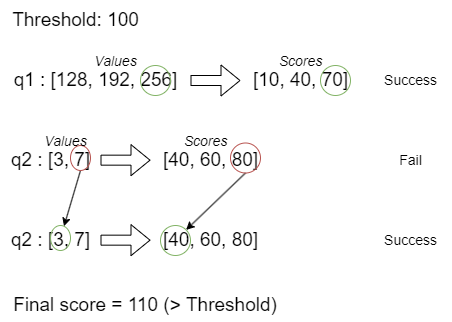
\includegraphics[scale=0.70]{images/Threshold_example.png}}
    \caption{Testing phase with threshold example}
    \label{fig:thex}
\end{figure}

\subsection{Discussion}
The first issue to address is the redundant re-certifications; specifically, it is important to filter out all the situations where configuration changes might happen on a device, but there is no way that such changes could influence the security certificate of the system. So, for example, if a device is updated with new features but is not actively communicating with other devices, it can be assumed that it is safe not to issue a certification process immediately. However, if such a device should send a message to another device for any reason, the certification process would be immediately needed, and it should be fast. Hence, to quickly release a certificate, it should be enough to certify only the involved features' security (such as the encryption and non-repudiation properties) and execute an extremely lightweight process to release a certificate with very limited validity (such as one hour or just one interaction). It is also possible to access the revoked certificates, check the process that allowed the certification to be completed first, and test the changes that caused the revocation; this way, the new certificate could benefit with a longer duration.

However, such an approach may not have a faster execution time than the current state-of-the-art techniques simply because those techniques imply that the execution phase is composed only of pre-defined test executions over well-aimed and known mechanisms. Therefore, the goal of the proposed solution approach is not to have a faster execution time; instead, it is to have a shorter and more automated overall certification process that would also require considerably fewer resources. Furthermore, directly mapping the properties and attributes to the tests that demonstrate them will be crucial to establishing the values of such attributes. In other words, defining a series of tests are important to determine if a given property or attribute is present. However, to do so efficiently, it is still necessary to have a set of device or system information that would allow the framework to filter out tests that are known to fail.


\subsection{Ephemeral Certificate Meaning}
The volatility or ephemerality of this approach comes from the fact that tests must be light and fast, hence, they cannot be in-depth and ensure a long lasting functioning of the system. (todo?)


\chapter{Experiments}
\label{cap4}
This chapter will illustrate an example of applying the proposed certification scheme to real software, showing how the manufacturer could benefit from such a solution.

\section{Certification Target}
The software considered for this demonstration is OpenSSL, a robust, commercial-grade, full-featured Open Source Toolkit for the Transport Layer Security (TLS) protocol formerly known as the Secure Sockets Layer (SSL) protocol. The protocol implementation is based on a full-strength general-purpose cryptographic library, which can also be used stand-alone.
OpenSSL is descended from the SSLeay library developed by Eric A. Young and Tim J. Hudson []. The OpenSSL crypto library (libcrypto) implements various cryptographic algorithms used in various Internet standards. The services provided by this library are used by the OpenSSL implementations of TLS and CMS, and they have also been used to implement many other third-party products and protocols.
The functionality includes symmetric encryption, public key cryptography, key agreement, certificate handling, cryptographic hash functions, cryptographic pseudo-random number generators, message authentication codes (MACs), key derivation functions (KDFs), and various utilities.

OpenSSL was considered for this demonstration for two main reasons:
\begin{description}
    \item[Open-Source] It is open-source software, which allows browsing through the code (mainly written in the C language) publicly available in the official GitHub repository (https://github.com/openssl/openssl) and inspecting all the previous versions of the software with the relative update changes.
    \item[Vulnerabilities] Researchers found multiple exposed vulnerabilities of the software during the various years of deployment; in this thesis work, only two of them will be considered for the sake of the example, the first identified by the Common Vulnerability Scoring System (CVSS) as [CVE-2014-0224] and the second as [CVE-2016-7798].
    
    \begin{itemize}
        \item {[CVE-2014-0224]} allowed man-in-the-middle attackers [] to use a zero-length master key in certain OpenSSL-to-OpenSSL communications and consequently hijack sessions or obtain sensitive information via a crafted TLS handshake, also known as "CCS Injection" vulnerability [].
        \item {[CVE-2016-7798]} was a vulnerability of the OpenSSL Ruby gem, which used the same initialization vector for multiple encryptions in a specific configuration; this allowed attackers to decipher encrypted messages easily [].

    \end{itemize}
\end{description}

OpenSSL is not a product certified by third-party certification authorities with schemes like Common Criteria, but it will be considered as if it was for this demonstration. With standard approaches, the presence of such vulnerabilities would trigger the certificate revocation, obliging the manufacturer to fix the vulnerability and re-certificate the software with a full certification process, costing a considerable amount of money and time; instead, the proposed scheme would allow performing a faster and cheaper re-certification.

\section{Process Walkthrough}
This section will illustrate a complete walkthrough of the proposed certification scheme over a system based on OpenSSL that has to go through the OpenSSL cryptolibrary update.

\subsection{Trigger Phase}
The bug that exposed the first vulnerability ([CVE-2014-0224]) consisted of a bad implementation of the DTLS handshake protocol [], which allowed bad actors to defeat any encryption algorithm used effortlessly; hence, the influenced property is the ability to manage cryptographic keys securely.

The bug allowed entities to accept the ChangeCipherSpec message at timings different from the intended ones; hence, the attribute of the property that will be considered is the timing of the CCS message, which must satisfy two conditions to be accepted: i) there are no fragments from the handshake uncompleted (e.g. certificate validation) and ii) the next message received is Finished.

The bug that exposed the second vulnerability ([CVE-2016-7798]) consisted of a bad implementation of the Ruby Openssl gem when using the AES algorithm in Galois/Counter Mode (GCM) [], which allowed each initialization vector to be used multiple times; this resulted in weak encryption of data. The issue was caused by the initialization vector being set before the key when it should have been set after it. The attributes considered in this process are the encryption algorithm (AES-GCM), the satisfaction of the requirement of having a different initialization vector every time and the correlated certificate signing algorithm, which is also affected by this issue.

It is important to note that both the vulnerabilities described above affect the system's confidentiality; hence, confidentiality will be the only macro-property considered.

After the system receives the update, the trigger component analyses the changes, comparing the old certificates with the updated properties and attributes and extracting the following properties and attributes:
\begin{itemize}
    \item Ability to execute cryptographic mechanisms of appropriate strength and performance
    \begin{itemize}
        \item AES-GCM conditions
        \item AES-GCM key length
    \end{itemize}
    \item Ability to perform authenticated encryption algorithms
    \begin{itemize}
        \item DTLS handshake conditions
    \end{itemize}
    \item Ability to verify digital signatures
    \begin{itemize}
        \item Signature algorithm and key length
    \end{itemize}

\end{itemize}

After listing the impacted properties and attributes and making them available through the Changes function, the trigger signals a manual operator that the process requires attention.

\subsection{Manual Revision Phase}
An expert manual operator accesses the properties and attributes through the Changes function and deals with three main tasks:
\begin{itemize}
    \item According to technological standards, the operator has to assign to each attribute a list of values; in this example, they are:
    \begin{itemize}
        \item {[1]} (satisfied or not) for the AES-GCM conditions
        \item {[128, 192, 256]} for the key length of the AES-GCM algorithm
        \item {[1]} (satisfied or not) for the DTLS handshake conditions
        \item {[\texttt{sha-1WithRSAEncryption, sha-224WithRSAEncryption, sha-256WithRSAEncryption, sha-384WithRSAEncryption, sha-512WithRSAEncryption}]} for the signature algorithm and key length
    \end{itemize}
    
    \item According to her assumed knowledge, he assigns a range of scores that directly map to the values of each attribute:
    \begin{itemize}
        \item {[20]} for the AES-GCM conditions
        \item {[5, 10, 20]s} for the key length of the AES-GCM algorithm
        \item {[20]} for the DTLS handshake conditions
        \item {[5, 10, 20, 50, 70]} for the signature algorithm and key length
    \end{itemize}
    
    \item According to her assumed knowledge, he assigns a score threshold to the impacted macro-properties; in this case, to the confidentiality macro-property, he assigns a threshold of 80 and a weight of 1 (the final weighted sum is ignored for this example).
\end{itemize}

\subsection{Score Computation and Testing}
At this point, the system must compute the minimum value needed by each attribute to reach the threshold with the minimum possible effort. In this case, since the threshold is 80, each attribute needs a score of 20 and will be tested for the corresponding value:
\begin{itemize}
    \item 1 for the AES-GCM conditions
    \item 256 for the key length of the AES-GCM algorithm
    \item 1 for the DTLS handshake conditions
    \item \texttt{sha-256WithRSAEncryption} for the signature algorithm and key length
\end{itemize}

If the system holds such requirements, then the certificate can be released.

All tests were executed on a virtual machine running Linux Ubuntu version 22.04.1 using a client-server setup.
For CVE-2014-0224 the server was tested with OpenSSL version 0.9.8y, known for being vulnerable to the CCS injection attack, and version 3.0.2, which implements the security patch to the vulnerability. Both server instances were initialized with the same commands:

First, it is required to generate a new key and a certificate on the server that will be used to establish a secure SSL/TLS connection with the following command:
"openssl req -x509 -newkey rsa:4096 -keyout key.pem -out cert.pem -days 365 -nodes"; the command req is used to create a self-signed test certificate with the argument x509, and the other arguments are: i) \textbf{newkey rsa:4096} generates a new private RSA key of size 4096 bits, ii) \textbf{keyout} copies the generated key into a file named key.pem, iii) \textbf{out} copies the generated certificate into a file named cert.pem, iv) \textbf{days} specifies the validity duration of the certificate and v) \textbf{nodes} avoids encrypting the generated private key.
Next, the server can be started using the following command:
"\texttt{openssl s\_server -key key.pem -cert cert.pem -accept 44330 -www}"; the command \textbf{s\_server} implements a generic SSL/TLS server which accepts connections from remote clients speaking SSL/TLS, and the arguments are: i) \textbf{key} specifies the private key to use, ii) \textbf{cert} specifies the certificate file to use, iii) \textbf{accept} specifies the port to listen on for connections, and iv) \textbf{www} sets the server to send a status message back to the client when it connects.

On the client side, executing a script designed to check if the server is vulnerable to the CCS injection exploit is sufficient; such a script is publicly available on [nmap.org website] and uses the open-source tool Nmap []. The script works by sending a '\textit{ChangeCipherSpec}' message out of order and checking whether the server returns a '\textit{UNEXPECTED\_MESSAGE}' alert record or not. Since a non-patched server would simply accept this message, the CCS packet is sent twice in order to force an alert from the server. The server is vulnerable if the alert type is different from '\textit{UNEXPECTED\_MESSAGE}'; the script is shown in appendix B []. The output provided by the script is the following for the vulnerable server test:  

\begin{verbatim}
Starting Nmap 7.80 ( https://nmap.org ) at 2022-09-17 19:23 CEST
Nmap scan report for localhost (127.0.0.1)
Host is up (0.00012s latency).

PORT      STATE SERVICE
44330/tcp open  unknown
| ssl-ccs-injection: 
|   VULNERABLE:
|   SSL/TLS MITM vulnerability (CCS Injection)
|     State: VULNERABLE
|     Risk factor: High
|      OpenSSL before 0.9.8za, 1.0.0 before 1.0.0m, and 1.0.1 before 1.0.1h
|      does not properly restrict processing of ChangeCipherSpec messages,
|      which allows man-in-the-middle attackers to trigger use of a zero
|      length master key in certain OpenSSL-to-OpenSSL communications, and
|      consequently hijack sessions or obtain sensitive information, via
|      a crafted TLS handshake, aka the "CCS Injection" vulnerability.
|           
|     References:
|       http://www.cvedetails.com/cve/2014-0224
|       https://cve.mitre.org/cgi-bin/cvename.cgi?name=CVE-2014-0224
|_      http://www.openssl.org/news/secadv_20140605.txt

Nmap done: 1 IP address (1 host up) scanned in 1.18 seconds
\end{verbatim}

and the following for the patched server test:
\begin{verbatim}
Starting Nmap 7.80 ( https://nmap.org ) at 2022-09-17 19:26 CEST
Nmap scan report for localhost (127.0.0.1)
Host is up (0.000079s latency).

PORT      STATE SERVICE
44330/tcp open  unknown

Nmap done: 1 IP address (1 host up) scanned in 0.17 seconds
\end{verbatim}

The test results show that the server running OpenSSL version 3.0.2 is no longer vulnerable to the CCS injection attack, while, with version 0.9.8y, the script highlights the presence of the vulnerability.


The test for CVE-2016-7798 was executed by replicating the bug using OpenSSL's Ruby gem; moreover, the execution was done using Ruby version 2.0.0p648, known for being affected by the bug, and Ruby version 3.1.0p0, which implements the security patch to the vulnerability. The scripts used for testing are shown in appendix \ref{IV}.The server does mainly three operations: i) waits for a message from the client, ii) encrypts the received message with the AES-256-GCM algorithm, always using the same key and iii) sends a hashed version of the encrypted message back to the client. Moreover, the server encrypts the messages setting a random initialization vector first and then the key, as suggested by [], to reproduce the bug. On the other hand, the client sends multiple times the same message to the server and counts the different ciphered texts received; the ciphered texts are extracted from the hashed texts and inserted into a set, which automatically filters out all the identical elements; the number of different ciphered texts is then the size of such set. Theoretically, the number of different ciphered texts should equal the number of sent messages.

The output of the server is the same in both versions:
\begin{verbatim}
>> Listening on port 44330
>> Received, encrypted and sent 1000000 messages
\end{verbatim}

The output resulting from the client connected to the vulnerable server is the following:
\begin{verbatim}
>> Sending 1000000 messages to the server...
>> All the messages encrypted by the server are equal
\end{verbatim}

and the output resulting from the client connected to the patched version is the following:
\begin{verbatim}
>> Sending 1000000 messages to the server...
>> The server sent 1000000 different ciphered texts
\end{verbatim}

The test proves that the vulerability is not present anymore in the patched version since the number of chiphered texts equal the number of sent messages.


The test of the algorithm AES-GCM with a key length of 256 bits was executed using a client-server setup with the Ruby language; the scripts used are shown in the appendix \ref{aes}. This test aimed to ensure the system's (server) capability to decrypt messages using the AES-256-GCM algorithm. Moreover, the test steps are as follows: i) the client encrypts a message using the AES-256-GCM algorithm and sends it to the server, ii) the server decrypts the message and sends it back to the client as plaintext and iii) the client compares the received plaintext with the original message; if all the messages are successfully decrypted the test is passed. The output of the test on the server-side is the following:
\begin{scriptsize}
\begin{verbatim}
Listening on port 44330

Received:  => 94c5710fdb955d3c785ce8b7dd13c27fdc1413478698bcb00b5165ce0d046aa46b042ca5d411d557
Decrypted: => Test message

Received:  => 2168638686b8306cfab0f91c78b539c5c6b2b691ce7653d8f9e88a475a32775702f2e383876c98b9
Decrypted: => Test message

Received:  => 94d7bcaae857db4f7cc6ced44e13002359f3945dbc2ebd8ecb60ab31eedb045855e96837355d4732
Decrypted: => Test message

Received:  => 76d28244ff06b9e4b5e6a7acffae823e8e7a3627c605ff19e19ab694a74cf6eae4cd339e5243ecef
Decrypted: => Test message

Received:  => a97de6ed0ae94ebaf7b50af087c27da8e5d71207266c00881bd5e399dbc154a422b02cf68728499e
Decrypted: => Test message
\end{verbatim}
\end{scriptsize}

and the output of the test on the client-side is the following:
\begin{verbatim}
The server decrypted the message correctly: { Test message }
The server decrypted the message correctly: { Test message }
The server decrypted the message correctly: { Test message }
The server decrypted the message correctly: { Test message }
The server decrypted the message correctly: { Test message }
The server decrypted all messages successfully!
\end{verbatim}

The output confirms the server's capability of decrypting messages with the AES-256-GCM algorithm.




The test of the sha-256WithRSAEncryption signature algorithm was also executed using a client-server setup with the Ruby language; the scripts used are shown in the appendix \ref{sig}. This test aimed to verify the integrity of the system's (server) certificate when generated using the sha-256WithRSAEncryption algorithm.The test's steps are as follows: i) the client connects to the server and sends an \textit{HELLO} message, ii) the server accepts the connection and replies to the \textit{HELLO} message with its certificate, iii) the client receives the server's certificate and extracts the server's public key from it, iv) the client uses the server's public key to encrypt a document and sends the result to the server, v) the server receives the encrypted document and decrypts it with its private key, vi) the server uses its private key to sign the decrypted document and sends the result to the client and vii) the client receives the signed document and verifies the authenticity of the signature usign the server's public key; if such verification succeeds the test is passed.

The output of the test on the server-side is the following:
\begin{verbatim}
>> Server listening on port 44330

>> New client connected

>> Received client's HELLO message, certificate sent

>> Received document encrypted by the client with this server's public key
>> Decrypted text:
This is an example document

>> Document signed with this server's private key

>> Signed document sent to the client

>> The client terminated the connection
\end{verbatim}

and the output of the test on the client-side is the following:
\begin{verbatim}
>> Connected to the server at 127.0.0.1:44330

>> HELLO message sent

>> Received server's certificate:
-----BEGIN CERTIFICATE-----
MIIFuzCCA6OgAwIBAgIUMo/2YlijMS2n80NQTCOWYPAg8UAwDQYJKoZIhvcNAQEL
BQAwbTELMAkGA1UEBhMCaXQxCzAJBgNVBAgMAnZhMRIwEAYDVQQHDAlnYWxsYXJh
dGUxDjAMBgNVBAoMBXVuaW1pMQ8wDQYDVQQDDAZtYXR0ZW8xHDAaBgkqhkiG9w0B
CQEWDXRlb0BnbWFpbC5jb20wHhcNMjIwOTIwMTU1MzAxWhcNMjMwOTIwMTU1MzAx
WjBtMQswCQYDVQQGEwJpdDELMAkGA1UECAwCdmExEjAQBgNVBAcMCWdhbGxhcmF0
ZTEOMAwGA1UECgwFdW5pbWkxDzANBgNVBAMMBm1hdHRlbzEcMBoGCSqGSIb3DQEJ
ARYNdGVvQGdtYWlsLmNvbTCCAiIwDQYJKoZIhvcNAQEBBQADggIPADCCAgoCggIB
ALi7TCyfIx9vJX4aofx0KlLwBctf+oKDn+xUduDJh43d31WvBGlomfUYxGGzlsWm
UXUaJ+mNf57kEra+zoIPVF2vIExr0CD7HpaYzRnWQGb5PFQkSppmfpMOzRTu94R+
7d47rMSNKY8g0G3gwhZMcVViBKUmDmoUccn1piW4s2Ur+esWfvb9qhBHJ8uqhL7h
2sFStjZKhIiMyW0zJcepnD9QikNme76X2fmYPS6pb7oMhdYurj4ILbqJctazmLMi
w2VLas74eVD9SA9WcszNIgNUBh7adTXHHPM9t6YGzYLGkn0PQ+vi5BqKPaTWdY8x
s6OFgh37klDPgvOAKDCVMRUkGSRzOpB/0k5wu6t9R6XY4mpa3BTxvEoee3B6Wx6z
WRJuemjx26JGw7D+enDXEw8+DCj532so1m0ytHKTrQd0NI5xztUJUdFE1e0/EnOR
m0Dq9/FYE1acpJnNo+FRApD1zcd08UdSF1DNNbVv27EVWCVHJFu7BlSl6tHvFroW
pSMkZtk2JVmkkAfrqJDdMhz7EZ65w9NSYy7DQEhYiYequnVei7lAHRVONJ3nQffw
EasNyDKG37WwarMFoqib4/8GDMtU0j/osQp9UAslMEBYQHFEakQRq8It5ACsznkw
AZy7ojZiQSkFdjqJ7cDyJhdiQcv9dKc0kIORKbZQ/17rAgMBAAGjUzBRMB0GA1Ud
DgQWBBTatWBPOpLFToMvhyV4q3vcRG+cQTAfBgNVHSMEGDAWgBTatWBPOpLFToMv
hyV4q3vcRG+cQTAPBgNVHRMBAf8EBTADAQH/MA0GCSqGSIb3DQEBCwUAA4ICAQA0
x7/Aab/6ZI7YVrwUZhkL49SfHQjP8aTtX2exJCN/IylYnlmdtf44PBYGSEK4dMP6
yCKPgtFTH1nFV/IndgQiy/bdyqGZa/wQmvP4lQp2AlyasTF+5uBmihdR7K11H+kA
8jdO2t0RqcVak+9M+F1uzCIAgu4fL2oMDwekfkI7ZBYYZdhMOdQItSJgN4bMJufj
UkzVwgy9q9UMEIRyCyXjI9HKF1rLYm7MtqBLBl90PT3jqgxqAgjOIaNQecg4pM1Z
PqVjHDSiIZwLvwdff59Aoaxiuq7lKk23A9RNcBGcv4dQCkzMWs4z6QL8pfNQJAL4
49iVcsSlxuYOtj3BCIO8+TJS+VBDiRljd3ekVFdObXrCeACGVm78sBXMmJH/UTFX
1kaJ4vkGblqlj2Ye3mpmc3H8qF3stRMv6dzWCJDggqA2NJI38Jc4u4/yXicrBmdv
6IwJe9JtYqJ5bRYE1Ig9Lb0y6SF7Hh4mIaKZGtwJgxf6jqIxuZAFM1Yv9S0wqUN+
78G+YsjA87T+6jHV1raXXTidGHGdPwYK/scQ7PvGUUk0Tl9YOagnxvbIeQRmNmLz
aj0YDPtAB0HJsqhZblVKqougfiRWyFaabnbunal5Vffs5BOfbDqIBFP5EZSCB0oS
fywDFN1Go/TGzqwrOrkwIE8S1PMs95es6qTZxzyJkQ==
-----END CERTIFICATE-----


>> Extracted server's public key:
-----BEGIN PUBLIC KEY-----
MIICIjANBgkqhkiG9w0BAQEFAAOCAg8AMIICCgKCAgEAuLtMLJ8jH28lfhqh/HQq
UvAFy1/6goOf7FR24MmHjd3fVa8EaWiZ9RjEYbOWxaZRdRon6Y1/nuQStr7Ogg9U
Xa8gTGvQIPselpjNGdZAZvk8VCRKmmZ+kw7NFO73hH7t3jusxI0pjyDQbeDCFkxx
VWIEpSYOahRxyfWmJbizZSv56xZ+9v2qEEcny6qEvuHawVK2NkqEiIzJbTMlx6mc
P1CKQ2Z7vpfZ+Zg9LqlvugyF1i6uPggtuoly1rOYsyLDZUtqzvh5UP1ID1ZyzM0i
A1QGHtp1Nccc8z23pgbNgsaSfQ9D6+LkGoo9pNZ1jzGzo4WCHfuSUM+C84AoMJUx
FSQZJHM6kH/STnC7q31HpdjialrcFPG8Sh57cHpbHrNZEm56aPHbokbDsP56cNcT
Dz4MKPnfayjWbTK0cpOtB3Q0jnHO1QlR0UTV7T8Sc5GbQOr38VgTVpykmc2j4VEC
kPXNx3TxR1IXUM01tW/bsRVYJUckW7sGVKXq0e8WuhalIyRm2TYlWaSQB+uokN0y
HPsRnrnD01JjLsNASFiJh6q6dV6LuUAdFU40nedB9/ARqw3IMobftbBqswWiqJvj
/wYMy1TSP+ixCn1QCyUwQFhAcURqRBGrwi3kAKzOeTABnLuiNmJBKQV2OontwPIm
F2JBy/10pzSQg5EptlD/XusCAwEAAQ==
-----END PUBLIC KEY-----


>> Encrypting the following document:
This is an example document

>> Encrypted document sent to the server

>> Received document signed with the server's private key

>> The server's signature is authentic

>> Connection terminated
\end{verbatim}

The output confirms the integrity of the server's certificate generated with the ha-256WithRSAEncryption signature algorithm.

\chapter{Conclusions}
\label{cap5}

\appendix
\chapter{Properties Taxonomy}
\label{taxonomy}
The NIST officially published several technical and non-technical capabilities that an IoT system’s manufacturer should consider; It should be noted that the following security requirements have been officially classified under one of the three parts of the CIA triad by the NIST.

Device identification, which is the capability to identify the IoT device for multiple purposes and in multiple ways to meet organizational requirements, is composed of the following requirements:

\begin{description}
    \item[Identifier Management Support] Ability for device identification. Elements that may be necessary:
        \begin{itemize}
            \item Ability to uniquely identify the IoT device logically.
            \item Ability to uniquely identify a remote IoT device.
            \item Ability for the device to support a unique device ID (e.g., to allow it to be linked to the person or process assigned to use the IoT device).
        \end{itemize}
    \item[Device Authentication Support] Ability to support local or interfaced device authentication. Elements that may be necessary:
        \begin{itemize}
            \item Ability for the IoT device to identify itself as an authorized entity to other devices.
            \item Ability to verify the identity of an IoT device.
        \end{itemize}
    \item[Physical Identifiers] Ability to add a unique physical identifier at an external or internal location on the device authorized entities can access.
\end{description}

On the other hand, the device configuration is defined as The capability to configure the IoT device through logical or physical interfaces to meet organizational requirements and includes the following requirements:
\begin{description}
    \item[Logical Access Privilege Configuration] Ability for only authorized entities to apply logical access privilege settings within the IoT device and configure logical access privilege as described in Logical Access to Interfaces.
    \item[Authentication and Authorization Configuration] Ability for only authorized entities to configure IoT device authentication policies and limitations as described in Logical Access to Interfaces.
    \item[Interface Configuration] Ability for only authorized entities to configure aspects related to the device’s interfaces as described in Logical Access to Interfaces.
    \item[Display Configuration] Ability to configure content to be displayed on a device.
    \item[Device Configuration Control] Ability to change configurations on the IoT device based on operational events as described in Device Security and Cybersecurity Event Awareness.
    \begin{itemize}
        \item Ability to change the device’s software configuration settings.
        \item Ability for authorized entities to restore the device to a secure configuration defined by an authorized entity.
        \item Configuration settings for use with the Device Configuration capability including, but not limited to:
        \begin{itemize}
            \item Ability for authorized entities to configure the cryptography use itself, such as choosing a key length.
            \item Ability to configure any remote update mechanisms to be either automatically or manually initiated for update downloads and installations.
            \item Ability to enable or disable notification when an update is available and specify who or what is to be notified.
        \end{itemize}
    \end{itemize}
\end{description}

Every IoT system revolves around data, and protecting it is the core focus of cybersecurity; the NIST defines data protection as the capability to protect IoT device data to meet organizational requirements. Therefore, it is important to satisfy as many of the following requirements as possible to achieve a high level of data protection.

\begin{description}
    \item[Cryptography Capabilities and Support] Ability for the IoT device to use cryptography for data protection. Elements that may be necessary:
        \begin{itemize}
            \item Ability to execute cryptographic mechanisms of appropriate strength and performance.
            \item Ability to obtain and validate certificates.
            \item Ability to verify digital signatures.
            \item Ability to run hashing algorithms.
            \item Ability to perform authenticated encryption algorithms.
            \item Ability to compute and compare hashes.
        \end{itemize}
    \item[Cryptographic Key Management] Ability to manage cryptographic keys securely:
        \begin{itemize}
            \item Ability to generate key pairs.
            \item Ability to store encryption keys securely.
            \item Ability to change keys securely.
        \end{itemize}
    \item[Secure Storage] Ability for the IoT device, or tools used through the IoT device interface, to enable secure device storage. Elements that may be necessary:
        \begin{itemize}
            \item Ability to support encryption of data at rest.
            \begin{itemize}
                \item Ability to cryptographically store passwords at rest, as well as device identity and other authentication data.
                \item Ability to support data encryption and signing to prevent data from being altered in device storage.
            \end{itemize}
            \item Ability to secure data in device storage
                \begin{itemize}
                    \item Ability to secure data stored locally on the device.
                    \item Ability to secure data stored in remote storage areas (e.g., cloud, server, etc.).
                    \item Ability to utilize separate storage partitions for system and user data.
                \end{itemize}
            \item Ability to “sanitize” or “purge” specific or all data in the device.
        \end{itemize}
        
    \item[Secure Transmission] Ability to secure data transmissions sent to and from the IoT device. Elements that may be necessary:
    \begin{itemize}
        \item Ability to configure the cryptographic algorithm to protect data in transit.
        \begin{itemize}
            \item Ability to support trusted data exchange with a specified minimum strength cryptography algorithm.
            \item Ability to support data encryption and signing to prevent data from being altered in transit.
        \end{itemize}
        \item Ability to utilize one or more capabilities to protect the data it transmits from unauthorized access and modification.
        \item Ability to use cryptographic means to validate the integrity of data transmitted.
    \end{itemize}
\end{description}

Another important aspect is the security of logical access to the system's interfaces, which is the ability to require authentication to or identify the IoT device and to establish authentication and identification configuration and display requirements.

\begin{description}
    \item[Authentication Support] Ability to support authentication methods.
    \begin{itemize}
        \item Ability for the IoT device to require authentication prior to connecting to the device.
        \item Ability for the IoT device to support and require appropriate authentication
        \begin{itemize}
            \item Ability for the IoT device to require authentication prior to connecting to the device.
            \item Ability for the IoT device to support a second, or more, authentication method(s) through an out of band path such as temporary passwords or other one-use logon credentials, third-party credential checks, biometrics, text messages, hard tokens and manufacturer proprietary methods
        \end{itemize}
        \item Ability for the IoT device to hide or mask authentication information during authentication process.
        \item Ability for the IoT device to support a second, or more, authentication method(s) through an out-of-band path such as: Temporary passwords or other one-use credentials; Third-party credential checks; Biometrics; Text messages; Hard Tokens; etc.
    \end{itemize}
    
    \item[Authentication Configuration] Ability to require, or not require, authentication to, and/or identification of, the IoT device, and to establish authentication and identification configuration and display requirements. Elements that may be necessary:
    \begin{itemize}
        \item Ability to set and change authentication configurations, policies and limitations settings for the IoT device
        \begin{itemize}
            \item Ability to set the time period for how long the device will remain locked after an established configurable limit of unsuccessful login attempts has been met.
            \item Ability to disable or lock access to the device after an established number of unsuccessful login attempts.
            \item Ability to display and/or report the previous date and time of the last successful login authentication.
            \item Ability to automatically disable accounts for the IoT device after an establish period of inactivity
            \item Ability to support automatic logout of inactive accounts after a configurable established time period.
            \item Ability to support automatic removal of temporary, emergency and other special use accounts after an established time period.
        \end{itemize}
        \item Ability to authenticate external users and systems
        \item Ability to revoke their access.
    \end{itemize}
    
    \item[System Use Notification Support] Ability to support system use notifications.
    \begin{itemize}
        \item Ability to display to IoT device users an organizationally-defined system use notification message or banner prior to successful IoT device authentication. (e.g., the message or banner would provide privacy and security notices consistent with applicable federal laws, Executive Orders, directives, policies, regulations, standards, and guidance).
        \item Ability to create an organizationally-defined system use notification message or banner to be displayed on the IoT device
        \begin{itemize}
            \item Ability to edit an existing IoT device display.
            \item Ability to establish the maximum size (in characters, bytes, etc.) of the available device display.
        \end{itemize}
        \item Ability to keep the notification message or banner on the device screen until the device user actively acknowledges and agrees to the usage conditions
    \end{itemize}
    
    \item[Authorization Support] Ability to restrict all unauthorized interactions.
    \begin{itemize}
        \item Ability to identify authorized users and processes.
        \item Ability to differentiate between authorized and unauthorized users (physical and remote).
    \end{itemize}
    
    \item[Authentication And Identity Management] Ability to establish access to the IoT device to perform organizationally-defined user actions without identification or authentication.
    
    
    \item[Role Support And Management] Ability to establish unique, privileged, organization-wide, and other types of IoT device user accounts. Elements that may be necessary:
    \begin{itemize}
        \item Ability to create unique IoT device user accounts.
        \item Ability to assign roles to IoT device user accounts.
        \item Ability to identify unique IoT device user accounts.
        \item Ability to support a hierarchy of logical access privileges for the IoT device based on roles (e.g., admin, emergency, user, local, temporary, etc.).
        \begin{itemize}
            \item Ability to establish user accounts to support role-based logical access privileges.
            \item Ability to administer user accounts to support role-based logical access privileges.
            \item Ability to use organizationally-defined roles to define each user account’s access and permitted device actions.
            \item Ability to support multiple levels of user/process account functionality and roles for the IoT device.
        \end{itemize}
        \item Ability to apply least privilege to user accounts (i.e., to ensure that the processes operate at privilege levels no higher than necessary to accomplish required functions).
        \begin{itemize}
            \item Ability to create additional processes, roles (e.g., admin, emergency, temporary, etc.) and accounts as necessary to achieve least privilege.
            \item Ability to apply least privilege settings within the device (i.e., to ensure that the processes operate at privilege levels no higher than necessary to accomplish required functions).
            \item Ability to limit access to privileged device settings that are used to establish and administer authorization requirements.
            \item Ability for authorized users to access privileged settings.
        \end{itemize}
        \item Ability to support organizationally-defined actions for the IoT device.
        \begin{itemize}
            \item Ability to create organizationally-defined accounts that support privileged roles with automated expiration conditions.
            \item Ability to establish organizationally-defined user actions for accessing the IoT device and/or device interface.
            \item Ability to enable automation and reporting of account management activities.
            \item Ability to assign access to IoT device audit controls to specific roles or organizationally-defined personnel.
            \item Ability to control access to IoT device audit data.
            \item Ability to identify the user, process or device requesting access to the audit/accountability information (i.e., to ensure only authorized users and/or devices have access).
            \item Ability to establish conditions for shared/group accounts on the IoT device.
            \item Ability to administer conditions for shared/group accounts on the IoT device.
            \item Ability to restrict the use of shared/group accounts on the IoT device according to organizationally-defined conditions.
        \end{itemize}
        \item Ability to implement dynamic access control approaches (e.g., service-oriented architectures) that rely on:
        \begin{itemize}
            \item run-time access control decisions facilitated by dynamic privilege management.
            \item organizationally-defined actions to access/use device.
        \end{itemize}
        \item Ability to allow information sharing capabilities based upon the type and/or role of user attempting to share the information.
        \item Ability to restrict access to IoT device software, hardware, and data based on user account roles, used with proper authentication of the identity of the user to determine type of authorization.
    \end{itemize}
    
    
    \item[Limitations on Device Usage] Ability to establish restrictions for how the device can be used. Elements that may be necessary:
    \begin{itemize}
        \item Ability to establish pre-defined restrictions for information searches within the device.
        \item Ability to establish limits on authorized concurrent device sessions for:
        \begin{itemize}
            \item User accounts
            \item Roles
            \item Groups
            \item Dates
            \item Times
            \item Locations
            \item Manufacturer established parameters
        \end{itemize}
    \end{itemize}
    
    
    \item[External Connections] Ability to support external connections. Elements that may be necessary:
    \begin{itemize}
        \item Ability to securely interact with authorized external, third-party systems.
        \item Ability to allow for the user/organization to establish the circumstances for when information sharing from the device and/or through the device interface will be allowed and prohibited.
        \item Ability to establish automated information sharing to approved identified parties/entities.
        \item Ability to identify when the external system meets the required security requirements for a connection.
        \item Ability to establish secure communications with internal systems when the device is operating on external networks.
    \end{itemize}
    
    \item[Interface Control] Ability to establish controls for the connections made to the IoT device. Elements that may be necessary:
    \begin{itemize}
        \item Ability to establish requirements for remote access to the IoT device and/or IoT device interface including:
        \begin{itemize}
            \item Usage restrictions
            \item Configuration requirements
            \item Connection requirements
            \item Manufacturer established requirement
        \end{itemize}
        \item Ability to restrict use of IoT device components (e.g., ports, functions, microphones, video).
        \item Ability to logically or physically disable any local and network interfaces that are not necessary for the core functionality of the device.
        \item Ability to restrict updating actions to authorized entities.
        \item Ability to restrict access to the cybersecurity state indicator to authorized entities.
        \item Ability to restrict use of IoT device services.
        \item Ability to enforce the established local and remote access requirements.
        \item Ability to prevent external access to the IoT device management interface.
        \item Ability to control the IoT device’s logical interface (e.g., locally or remotely).
        \item Ability to change IoT device logical interface(s).
        \item Ability to control device responses to device input.
        \item Ability to control output from the device.
        \item Ability to support wireless technologies needed by the organization (e.g., Microwave, Packet radio (UHF/VHF), Bluetooth, Manufacturer defined)
        \item Ability to support communications technologies (including but not limited to):
        \begin{itemize}
            \item IEEE 802.11
            \item Bluetooth
            \item Ethernet
            \item Manufacturer defined
        \end{itemize}
        \item Ability to establish and configure IoT device settings for wireless technologies including authentication protocols (e.g., EAP/TLS, PEAP).
    \end{itemize}
\end{description}
    
    Given the intrinsic dynamicity of IoT systems and devices, software updates are frequent, and support mechanisms may need additional security properties. These requirements refer to the ability to update IoT device software and support mechanisms for such updates.
    \begin{description}
        \item[Update Capabilities] Ability to update the IoT device software within the device and/or through the IoT device interface. Elements that may be necessary:
        \begin{itemize}
            \item Ability to update the software by authorized entities only using a secure and configurable mechanism.
            \item Ability to identify the current version of the organizational audit policies and procedures governing the software update.
            \item Ability to restrict software installations to only authorized individuals or processes.
            \item Ability to restrict software changes/uninstallations to only authorized individuals or processes.
            \item Ability to verify software updates come from valid sources using an effective method (e.g., digital signatures, checksums, certificate validation, etc).
        \end{itemize}
        
        \item[Update Application Support] Ability to update the device’s software through remote (e.g., network download) and/or local (e.g., removable media) means
        \begin{itemize}
            \item If software updates are delivered and applied automatically:
            \begin{itemize}
                \item Ability to verify and authenticate any update before installing it
                \item Ability to enable or disable updating
            \end{itemize}
        \end{itemize}
    \end{description}
    
    
    %% skipping cybersecurity awareness %%
    
    Last but not least important is the device's security, defined as the capability to secure the IoT device to meet organizational requirements.
    
    \begin{description}
        \item[Secure Execution] Ability to protect the execution of code on the device. Elements that may be necessary:
        \begin{itemize}
            \item Ability to enforce organizationally-defined execution policies.
            \begin{itemize}
                \item Ability to execute code in confined virtual environments.
                \item Ability to separate IoT device processes into separate execution domains.
            \end{itemize}
            \item Ability to separate the levels of IoT device user functionality.
            \item Ability to authorize various levels of IoT device functionality.
        \end{itemize}
        
        
        \item[Secure Communication] Ability to securely initiate and terminate communications with other devices. Elements that may be necessary:
        \begin{itemize}
            \item Ability to enforce traffic flow policies.
            \item Ability to utilize standardized protocols.
            \item Ability to establish network connections.
            \item Ability to terminate network connections (e.g., automatically based on organizationally-defined parameters).
            \item Ability to de-allocate TCP/IP address/port pairings.
            \item Ability to establish communications channels.
            \item Ability to secure the communications channels.
            \item Ability to interface with DNS/DNSSEC.
            \item Ability to store and process session identifiers.
            \item Ability to identify and track sessions with identifiers.
        \end{itemize}
        
        \item[Secure Resource Usage] Ability to securely utilize system resources and memory. Elements that may be necessary:
        \begin{itemize}
            \item Ability to support shared system resources.
            \begin{itemize}
                \item Ability to release resources back to the system.
                \item Ability to separate user and process resources use.
                \item Ability to no one will read this.
            \end{itemize}
            \item Ability to manage memory address space assigned to processes.
            \item Ability to enforce access to memory space through the kernel.
            \item Ability to prevent a process from accessing memory space of another process.
            \item Ability to enforce configured disk quotas.
            \item Ability to continue operation when associated networks are unavailable (e.g., a smart smoke detector must still go off when a fire occurs even if it is not attached to the associated network).
            \item Ability to provide sufficient resources to store and run the operating environment (e.g., operating systems, firmware, applications).
            \item Ability to utilize file compression technologies (e.g., to provide denial of service protection).
        \end{itemize}
        
        
        \item[Device Integrity] Ability to protect against unauthorized changes to hardware and software. Elements that may be necessary:
        \begin{itemize}
            \item Ability to perform security compliance checks on system components.
            \item Ability to detect unauthorized hardware and software components.
            \item Ability to take organizationally-defined actions when unauthorized hardware and software components are detected (e.g., disallow a flash drive to be connected even if a USB port is present).
            \item Ability to store the operating environment (e.g., firmware image, software, applications) in read-only media (e.g., Read Only Memory).
        \end{itemize}
        
        \item[Secure Device Operation] Ability to operate securely and safely. Elements that may be necessary:
        \begin{itemize}
            \item Ability to keep an accurate internal system time.
            \item Ability to define various operational states.
            \item Ability to support various modes of IoT device operation with more restrictive operational states.
            \begin{itemize}
                \item “travel mode” for transit.
                \item “safe mode” for operation when some or all network security is unavailable.
                \item Others as determined necessary based on the purpose and goals for the IoT device.
            \end{itemize}
            \item Ability to define differing failure types.
            \item Ability to fail in a secure state.
            \item Ability to disable operations and/or functionality in the event of security violations.
            \item Ability to restrict components/features of the IoT device (e.g., ports, functions, protocols, services, etc.) in accordance with organizationally-defined policies.
            \item Ability to sense the environment and securely (i.e., preserving confidentiality, integrity, and availability of the device and its data) interface with the environment, either directly or through the IoT system. Examples include:
            \begin{itemize}
                \item Emergency shutoff mechanism
                \item Emergency lighting mechanism
                \item Fire protection mechanism
                \item Temperature and humidity mechanism
                \item Water damage protection mechanism
                \item Manufacturer defined capability
            \end{itemize}
        \end{itemize}
        
        
    \end{description}
    
    
    Moreover, Nasiri et al. \cite{nasiri2019security} defined a series of security requirements that manufacturers should consider (and develop) when designing IoT systems. These requirements are a high-level summary of the above that could be useful while showcasing examples of systems’ design. Although the research refers to healthcare IoT systems, many properties are still relevant for any kind of IoT system.
    
    \begin{description}
        \item[Identification and authentication] Identification guarantees the identity of all the entities before permitting them to interact with the resources of the IoT system. Authentication is the process of confirming the identity of a person or device before using the system resources. Devices and application authentication can prove that the interacting system is not an adversary and that data shared in networks is legal.
        
        \item[authorization (access control)] After user identity verification, access rights or privileges to resources should be determined so that different users can only access the resources required based on their tasks.

        \item[privacy] Privacy means that secrets and personal data of users should not be disclosed without consent. Therefore, the IoT system should be in accordance with privacy policies allowing users to control their private data.

        \item[accountability] In a health IoT system, accountability should ensure that the organization or individuals are obliged to be answerable or responsible for their actions in case of theft or abnormal event.

        \item[non-repudiation] Non-repudiation ensures that someone cannot deny an action that has already been done. It enables the users to prove the occurrence or non-occurrence of an event.

        \item[auditing] Auditing is the ability of a system to track and monitor actions continuously. All user activities should be recorded in sequential order, such as system login time and data modification.
        
        \item[data freshness] Data freshness means that data should be recent, ensuring that no old messages are replayed.

        

    \end{description}
    

\chapter{Scripts Used For Testing}
\section{CCS Injection Nmap Script}
\label{ccs}
\lstinputlisting[basicstyle=\footnotesize]{Files/ssl-ccs-injection}

\section{CVE-2016-779 Ruby Scripts}
\label{IV}
\textbf{Server}
\label{iv_server}
\lstinputlisting[basicstyle=\footnotesize, language=Ruby]{Files/IV/server.rb}
\textbf{Client}
\label{iv_client}
\lstinputlisting[basicstyle=\footnotesize, language=Ruby]{Files/IV/client.rb}

\newpage
\section{Signature Algorithm Ruby Scripts}
\label{sig}
\textbf{SocketIO}
\label{sig_io}
\lstinputlisting[basicstyle=\footnotesize, language=Ruby]{Files/Sig/socketIO.rb}
\textbf{Server}
\label{sig_server}
\lstinputlisting[basicstyle=\footnotesize, language=Ruby]{Files/Sig/server.rb}
\textbf{Client}
\label{sig_client}
\lstinputlisting[basicstyle=\footnotesize, language=Ruby]{Files/Sig/client.rb}

\section{AES-256-GCM Algorithm Ruby Scripts}
\label{aes}
\textbf{Server}
\label{aes_server}
\lstinputlisting[basicstyle=\footnotesize, language=Ruby]{Files/Sig/server.rb}
\textbf{Client}
\label{aes_client}
\lstinputlisting[basicstyle=\footnotesize, language=Ruby]{Files/Sig/client.rb}

%
%			BIBLIOGRAFIA
%
\begin{thebibliography}{00}

\bibitem{mell2011nist}Mell, P., Grance, T. \& Others The NIST definition of cloud computing. (Computer Security Division, Information Technology Laboratory, National …,2011)

\bibitem{atlam2017integration}Atlam, H., Alenezi, A., Alharthi, A., Walters, R. \& Wills, G. Integration of cloud computing with internet of things: challenges and open issues. {\em 2017 IEEE International Conference On Internet Of Things (iThings) And IEEE Green Computing And Communications (GreenCom) And IEEE Cyber, Physical And Social Computing (CPSCom) And IEEE Smart Data (SmartData)}. pp. 670-675 (2017)

\bibitem{khan2019edge}Khan, W., Ahmed, E., Hakak, S., Yaqoob, I. \& Ahmed, A. Edge computing: A survey. {\em Future Generation Computer Systems}. \textbf{97} pp. 219-235 (2019)

\bibitem{gokhale2018introduction}Gokhale, P., Bhat, O. \& Bhat, S. Introduction to IOT. {\em International Advanced Research Journal In Science, Engineering And Technology}. \textbf{5}, 41-44 (2018)

\bibitem{iorga2018fog}Iorga, M., Feldman, L., Barton, R., Martin, M., Goren, N., Mahmoudi, C. \& Others Fog computing conceptual model.  (2018)

\bibitem{sahni2018data}Sahni, Y., Cao, J. \& Yang, L. Data-aware task allocation for achieving low latency in collaborative edge computing. {\em IEEE Internet Of Things Journal}. \textbf{6}, 3512-3524 (2018)

\bibitem{yi2015fog}Yi, S., Hao, Z., Qin, Z. \& Li, Q. Fog computing: Platform and applications. {\em 2015 Third IEEE Workshop On Hot Topics In Web Systems And Technologies (HotWeb)}. pp. 73-78 (2015)

\bibitem{atlam2018fog}Atlam, H., Walters, R. \& Wills, G. Fog computing and the internet of things: A review. {\em Big Data And Cognitive Computing}. \textbf{2}, 10 (2018)

\bibitem{heck2010software}Heck, P., Klabbers, M. \& Eekelen, M. A software product certification model. {\em Software Quality Journal}. \textbf{18}, 37-55 (2010)

\bibitem{anisetti2017semi}Anisetti, M., Ardagna, C., Damiani, E. \& Gaudenzi, F. A semi-automatic and trustworthy scheme for continuous cloud service certification. {\em IEEE Transactions On Services Computing}. \textbf{13}, 30-43 (2017)

\bibitem{aslam2020fonac}Aslam, M., Mohsin, B., Nasir, A. \& Raza, S. FoNAC-an automated fog node audit and certification scheme. {\em Computers \& Security}. \textbf{93} pp. 101759 (2020)


\bibitem{baldini2016security}Baldini, G., Skarmeta, A., Fourneret, E., Neisse, R., Legeard, B. \& Le Gall, F. Security certification and labelling in Internet of Things. {\em 2016 IEEE 3rd World Forum On Internet Of Things (WF-IoT)}. pp. 627-632 (2016)

\bibitem{ardagna2015security}Ardagna, C., Asal, R., Damiani, E. \& Vu, Q. From security to assurance in the cloud: A survey. {\em ACM Computing Surveys (CSUR)}. \textbf{48}, 1-50 (2015)

\bibitem{infrastructure2002common}Infrastructure, P. \& Profile, T. Common criteria for information technology security evaluation. {\em National Security Agency}. (2002)

\bibitem{anisetti2013test}Anisetti, M., Ardagna, C., Damiani, E. \& Saonara, F. A test-based security certification scheme for web services. {\em ACM Transactions On The Web (TWEB)}. \textbf{7}, 1-41 (2013)

\bibitem{CSATrustSTAR}Cloud Security Alliance, Security CSATrust \& Assurance Registry (STAR). (\url{https://cloudsecurityalliance.org/star/}), Accessed: 2022-08-29

\bibitem{IBMConfChange}Configuration Change Overview. (\url{https://www.ibm.com/docs/en/mfnp/7.6.0?topic=changes-configuration-change-overview}), Accessed: 2022-08-29

\bibitem{mateusz2022flex}Mateusz Ciok, K., Pascual Espada, J. \& González Crespo, R. Flex-request: Library to make remote changes in the communication of IoT devices. {\em Expert Systems}. pp. e12994 (2022)

\bibitem{kaluvuri2014quantitative}Kaluvuri, S., Bezzi, M. \& Roudier, Y. A quantitative analysis of common criteria certification practice. {\em International Conference On Trust, Privacy And Security In Digital Business}. pp. 132-143 (2014)

\bibitem{keblawi2006applying}Keblawi, F. \& Sullivan, D. Applying the common criteria in systems engineering. {\em IEEE Security \& Privacy}. \textbf{4}, 50-55 (2006)

\bibitem{ICSAFw}Labs, I. ICSA Labs IoT Security Testing Framework. (\url{https://www.icsalabs.com/technology-program/iot-testing}), Accessed: 2022-08-29

\bibitem{surveyIOT}Matheu, S., Hernández-Ramos, J., Skarmeta, A. \& Baldini, G. A Survey of Cybersecurity Certification for the Internet of Things. {\em ACM Comput. Surv.}. \textbf{53} (2020,12), https://doi.org/10.1145/3410160

\bibitem{orangeBook}Latham, D. Department of defense trusted computer system evaluation criteria. {\em Department Of Defense}. \textbf{198} (1986)

\bibitem{ITSEC}Jahl, C. The information technology security evaluation criteria. {\em Proceedings-13th International Conference On Software Engineering}. pp. 306-307 (1991)

\bibitem{orangeBookDeath}Lipner, S. The birth and death of the orange book. {\em IEEE Annals Of The History Of Computing}. \textbf{37}, 19-31 (2015)

\bibitem{CTCPEC}Bacic, E. The Canadian trusted computer product evaluation criteria. {\em [1990] Proceedings Of The Sixth Annual Computer Security Applications Conference}. pp. 188-196 (1990)

\bibitem{CCProducts}Common Criteria Certified Products. (https://www.commoncriteriaportal.org/products/), Accessed: 2022-08-29

\bibitem{ardagna2014management}Ardagna, C., Asal, R., Damiani, E. \& Vu, Q. On the management of cloud non-functional properties: The cloud transparency toolkit. {\em 2014 6th International Conference On New Technologies, Mobility And Security (NTMS)}. pp. 1-4 (2014)

\bibitem{goertzel2007software}Goertzel, K., Winograd, T., McKinley, H., Oh, L., Colon, M., McGibbon, T., Fedchak, E. \& Vienneau, R. Software security assurance: a state-of-art report (sar). (INFORMATION ASSURANCE TECHNOLOGY ANALYSIS CENTER (IATAC) HERNDON VA,2007)

\bibitem{article}Ardagna, C., Asal, R., Damiani, E. \& Vu, Q. From Security to Assurance in the Cloud. {\em ACM Computing Surveys}. \textbf{48} pp. 1-50 (2015,7)

\bibitem{mahmud2018fog}Mahmud, R., Kotagiri, R. \& Buyya, R. Fog computing: A taxonomy, survey and future directions. {\em Internet Of Everything}. pp. 103-130 (2018)

\bibitem{macneil2006comply}MacNeil, I. \& Li, X. “Comply or Explain”: market discipline and non-compliance with the Combined Code. {\em Corporate Governance: An International Review}. \textbf{14}, 486-496 (2006)

\bibitem{anisetti2022multi}Anisetti, M., Ardagna, C. \& Bena, N. Multi-Dimensional Certification of Modern Distributed Systems. {\em IEEE Transactions On Services Computing}. (2022)

\bibitem{chen2013verification}Chen, M., Tan, T., Sun, J., Liu, Y., Pang, J. \& Li, X. Verification of functional and non-functional requirements of web service composition. {\em International Conference On Formal Engineering Methods}. pp. 313-328 (2013)

\bibitem{pub2005minimum}Pub, F. Minimum security requirements for federal information and information systems.  (2005)

\bibitem{nasiri2019security}Nasiri, S., Sadoughi, F., Tadayon, M. \& Dehnad, A. Security requirements of internet of things-based healthcare system: a survey study. {\em Acta Informatica Medica}. \textbf{27}, 253 (2019)

\bibitem{daemen1999aes}Daemen, J. \& Rijmen, V. AES proposal: Rijndael. (Gaithersburg, MD, USA,1999)

\bibitem{fischer2017dod}Fischer, T. DoD 5220.22-m data wipe method [US DOD wipe standard]. (Retrieved from Lifewire: https://www. lifewire. com/dod-5220-22-m-2625856,2017)

\bibitem{OpenSSLMan}Young, E. \& Hudson, T. OpenSSL Manual. , (\url{https://www.openssl.org/docs/man3.0/man7/crypto.html}), Accessed: 2022-09-13


\end{thebibliography}
% 
\end{document}


 
